\documentclass[12pt,MSc,wordcount,twoside,anon]{muthesis}
\usepackage[T1]{fontenc}
\usepackage[authoryear]{natbib}
\bibliographystyle{apalike} 

\usepackage{verbatim}
\usepackage{enumitem}
\setlist[itemize]{itemsep=2pt, topsep=4pt, parsep=0pt, partopsep=0pt}
\usepackage{graphicx}
\usepackage{url}
\usepackage{listings}
\usepackage{amsmath}
\usepackage{amssymb}
\usepackage{mathtools}
\usepackage{amsthm}
\usepackage{pslatex}
\usepackage[pdfusetitle=false, bookmarks=false]{hyperref}
\usepackage{cleveref}
\usepackage{tikz}
\usetikzlibrary{arrows.meta, shapes, positioning, fit, backgrounds}
\graphicspath{{./figures/}{../notebooks/}}

\newtheorem{theorem}{Theorem}[chapter]
\newtheorem{lemma}[theorem]{Lemma}
\newtheorem{corollary}[theorem]{Corollary}
\newtheorem{proposition}[theorem]{Proposition}

\theoremstyle{definition}
\newtheorem{definition}[theorem]{Definition}
\newtheorem{assumption}{Assumption}[chapter]
\newtheorem{example}[theorem]{Example}

\theoremstyle{remark}
\newtheorem{remark}[theorem]{Remark}

\DeclareMathOperator*{\argmin}{arg\,min}
\DeclareMathOperator*{\argmax}{arg\,max}

\setcounter{secnumdepth}{3}

\begin{document}

\title{Robust Variational Inference \\
via Imprecise Probabilities}

\stuid{11433615}

\principaladviser{Dr.Michele Caprio}


\beforeabstract

\prefacesection{Abstract}

\abstracttitle
{\singlespacing
Bayesian inference requires the specification of a prior 
distribution, yet in practice multiple priors are often 
equally defensible and the resulting posteriors can differ 
substantially under limited data. This thesis develops a 
principled framework for robust Bayesian inference under 
prior uncertainty, grounded in the theory of imprecise 
probabilities and realised computationally through flow 
matching. The central theoretical contribution is a 
guarantee that a credal mixture over $K$ flow-based 
posterior approximations achieves predictive performance 
no worse than the best single-prior component: the 
convexity of KL divergence ensures that combination over 
a credal set can only improve over selection. An 
approximate version of this guarantee is established for 
the practical setting where posteriors are learned by a 
shared-backbone conditional flow matching model and 
mixture weights are selected by held-out negative 
log-likelihood optimisation on the probability simplex.

The framework is evaluated through a systematic 
experimental programme spanning two real-world Bayesian 
classification datasets, a regression dataset, and three 
synthetic settings, with eight weight optimisation 
algorithms compared across multiple random seeds. Three 
pre-registered hypotheses are confirmed: the convexity 
guarantee is empirically visible in the prior-sensitive 
low-data regime, disappears correctly when data is 
sufficient to overwhelm prior influence, and the EM 
algorithm achieves the lowest worst-case regret among 
all algorithms tested. The credal mixture achieves 
near-oracle robustness with a factor of eight 
improvement in worst-case regret over the best 
val-selected single-prior strategy. A shared-backbone 
architecture is shown to outperform independently 
trained flows on predictive performance, training 
stability, and parameter efficiency, providing empirical 
validation for the uniform transfer assumption 
underpinning the theoretical guarantee.
}

\afterabstract

\prefacesection{Acknowledgements}
I would like to express my sincere gratitude to my 
supervisor, Dr.\ Michele Caprio, for his invaluable 
guidance, generosity with his time, and for 
contributing two important theoretical results 
to this thesis. His insight and encouragement 
throughout this project have been indispensable.

I am deeply grateful to my family for their 
unwavering support and for always believing in me, 
and to my girlfriend for her patience, 
understanding, and encouragement during the most 
demanding stretches of this work.

Finally, I would like to thank my cat Ash, whose 
companionship during the long hours of research 
and writing was a source of comfort that should 
not go unacknowledged.

\afterpreface

% These include the actual text
\chapter{Introduction}
\label{cha:intro}

\section{Background and Motivation}
Bayesian inference provides a rigorous framework for updating beliefs 
about model parameters in the light of observed data, yet the uncertainty 
it quantifies is not immune to uncertainty itself. This is the problem of 
second-order uncertainty, which arises because Bayesian inference carries a 
foundational assumption that the prior distribution is known and correctly 
specified. When multiple priors are equally plausible, committing to a single 
one is epistemically insufficient and can lead to overconfident inferences. 
The framework is precise about uncertainty over parameters but it fails to 
capture the uncertainty about the choice of the prior which precedes inference 
at the level of modelling itself. This problem has been recognised in the 
philosophy of probability since at least the 1960s, formalised under the 
study of imprecise probabilities and credal sets. Imprecise probability theory 
replaces the single prior distribution with a credal set, a convex set of 
distributions representing the range of plausible beliefs, and asks what 
conclusions are robust across the entire set rather than what is optimal 
under a single prior \citep{walley1991}\citep{wheeler2022}. This is a philosophically 
distinct response to the problem of second-order uncertainty. Rather than 
resolving prior uncertainty by collapsing it to a point, the framework carries 
that uncertainty forward explicitly into the inferential conclusions. The 
computational challenges of working with sets of distributions are formidable, 
however, and the focus on scalability in modern machine learning has led to 
the problem of second-order uncertainty being largely neglected.

Prior sensitivity is a routine challenge in Bayesian inference. When data 
is scarce, the likelihood is not sufficiently informative to overwhelm the 
influence of the prior and the posterior remains sensitive to the initial 
modelling choices. In settings such as healthcare, ecological modelling, or 
scientific parameter estimation, data is expensive to obtain or inherently 
limited; two practitioners using equally defensible priors can arrive at 
substantially different posteriors and therefore different conclusions. In a 
clinical trial setting, for instance, a sceptical prior and an optimistic 
prior over treatment efficacy can produce posteriors that disagree 
substantially about whether a drug should be recommended, not because the 
data is ambiguous, but because the prior is doing significant inferential 
work that is never formally acknowledged \citep{berger1994}. This sensitivity 
is not confined to small data or traditional statistical settings. Recent 
work has shown that prior choice remains consequential in deep Bayesian 
models; standard priors used in Bayesian neural networks are poorly 
calibrated and performance is sensitive to prior specification even at 
scale \citep{fortuin2021}, and cold posteriors, which correspond to 
implicitly rescaled priors, have been shown to outperform standard 
posteriors in deep learning settings \citep{wenzel2020}. Prior 
uncertainty is therefore not a historical concern that modern methods 
have resolved but an active and open problem in probabilistic machine 
learning.

Variational Inference (VI) has emerged as a powerful tool for Bayesian 
computation, offering a scalable alternative to Markov Chain Monte Carlo 
(MCMC) methods. However, standard VI inherits the same foundational 
limitation: it approximates a single posterior under a fixed prior, leaving 
second-order uncertainty unaddressed. VI is nevertheless a natural framework 
for operationalising credal sets at scale: rather than running a separate 
inference procedure for each candidate prior independently, one can train a 
family of variational posteriors jointly and combine them into a credal 
mixture, directly representing the uncertainty that a single posterior cannot 
capture. The computational challenge is making this tractable; training 
expressive posterior approximations across a set of priors simultaneously 
demands a flexible and scalable variational family.

Recent advances in normalising flows and their continuous-time generalisation 
through neural ordinary differential equations \citep{chen2018} have made 
expressive posterior approximation tractable. Flow matching \citep{lipman2022} represents a further step, replacing the computationally expensive 
log-determinant evaluations required by classical normalising flows with a 
direct regression objective over a learned velocity field. Crucially, the 
velocity field can be conditioned on auxiliary information, in this case a 
discrete prior index, at minimal additional cost, allowing a single shared 
model to approximate posteriors across all candidate priors simultaneously. 
This makes flow matching particularly well suited to the credal mixture 
setting and addresses the computational challenge directly.

This thesis investigates whether credal mixtures of flow-based posteriors 
can provide robust inference under prior uncertainty. The approach is grounded 
in a classical result from information theory: the KL divergence is convex 
in its second argument, which guarantees in principle that a mixture over a 
set of posteriors performs at least as well as the best individual component 
\citep{cover2006}. Whether this guarantee remains empirically visible 
under deep variational approximation, and what architectural and methodological 
conditions are required for it to hold, is the central question this work 
addresses.

\section{Existing Approaches to Prior Robustness}

Several approaches have been proposed to address the problem of prior 
sensitivity in Bayesian inference and to operationalise the concept of 
robustness to prior uncertainty. Each offers a different perspective on 
the problem and a different set of trade-offs, but none provides a 
principled treatment of second-order uncertainty in the sense formalised 
by imprecise probability theory.

\subsection{Epsilon-Contamination and Prior Classes}

The original formal treatment of prior robustness models the prior as 
belonging to an epsilon-contamination class, a convex set of distributions 
formed by mixing a baseline prior with an arbitrary contaminating 
distribution within some neighbourhood (Berger, 1984; Insua and Ruggeri, 
2000). Posterior bounds are then derived that hold for any prior in the 
class, providing a formal framework for analysing the sensitivity of 
inferences to perturbations of the prior. This is the intellectual 
precursor to the credal set approach and establishes the core idea that 
working with a class of priors rather than a single one is both principled 
and tractable. The limitation is that the prior class is defined 
analytically and the resulting posterior bounds are derived through 
closed-form calculations, which restricts applicability to simple models 
and low-dimensional settings. This approach does not scale to modern 
machine learning problems with high-dimensional parameter spaces and 
complex likelihoods.

\subsection{Gamma-Minimax Decision Theory}

Rather than committing to one prior, the gamma-minimax framework minimises 
the maximum expected loss over a class of priors, producing decisions that 
are robust to the worst-case prior within the class \citep{berger1985}. This 
is philosophically aligned with the imprecise probability approach in that 
it acknowledges a set of plausible priors rather than a single one. 
However, the minimax framing collapses the set at decision time: the 
output is a single decision that hedges against the worst case, rather 
than a set of posteriors that carries prior uncertainty forward. The 
second-order uncertainty is acknowledged in the decision procedure but 
is not propagated through inference in a way that allows downstream 
conclusions to reflect it.

\subsection{Bayesian Model Averaging}

Bayesian model averaging (BMA) combines a discrete set of candidate 
models or priors by weighting each according to its marginal likelihood 
\citep{hoeting1999}. This is the closest classical precursor to the 
credal mixture approach and is important to engage with carefully. The 
key distinction is that BMA uses marginal likelihood weights, which are 
themselves computed under each model's prior and collapsed into a single 
weighted predictive distribution. The weights are point estimates and the 
resulting average is a single distribution rather than a credal set. There 
is no formal commitment to representing the uncertainty across the set; 
BMA resolves prior uncertainty by weighting rather than carrying it forward. 
Furthermore, marginal likelihood weights can be dominated by a single model 
when one prior fits the data substantially better, which may not reflect 
genuine robustness across the set.

\subsection{Stacking of Predictive Distributions}

Stacking fits mixture weights over a set of candidate posteriors by 
maximising held-out log predictive scores, making it the most directly 
related existing method to the approach developed in this thesis \citep{yao2018}. Operationally, stacking shares the combination mechanism: 
a set of posteriors is trained and weights are selected using a 
likelihood-consistent objective. However, stacking treats the candidate 
models as fixed and selects weights purely for predictive performance, 
without any theoretical grounding in imprecise probability theory or the 
KL convexity guarantee. It is a pragmatic ensemble method rather than 
a principled treatment of second-order uncertainty. The mixture weights 
in stacking are justified by cross-validated predictive accuracy alone; 
in the credal mixture framework developed here, the combination is 
grounded in the convexity of KL divergence, which provides a theoretical 
guarantee that the mixture performs at least as well as the best 
individual component.

\subsection{Generalised Bayesian Inference}

Generalised Bayesian inference replaces the likelihood in Bayes' rule 
with a general loss function, producing a family of posteriors indexed 
by the loss rather than a single posterior \citep{bissiri2016}. 
Knoblauch et al. \citep{knoblauch2022} extend this framework and explicitly discuss 
robustness to both prior and likelihood misspecification as a unified 
problem, making this the most theoretically sophisticated modern approach 
to Bayesian robustness. The framework implicitly defines a set of 
plausible posteriors under different modelling assumptions, which is 
conceptually adjacent to the credal set idea. However, it does not 
formally invoke imprecise probability theory; it does not treat the 
resulting set of posteriors as a credal set or ask what can be concluded 
robustly across it. It produces alternative posteriors rather than 
representing and propagating genuine second-order uncertainty, and it 
does not provide a mechanism for combining posteriors across a set 
of priors in a principled way.

\subsection{Robust Divergence-Based Variational Inference}

Robust divergence-based variational inference replaces the KL divergence 
in the VI objective with a more robust alternative such as the 
beta-divergence or gamma-divergence, achieving resistance to outliers 
and likelihood misspecification \citep{futami2018, knoblauch2019}. While superficially related to the goal of robust inference, 
this approach addresses a fundamentally different problem. It produces 
a single posterior under a single prior, changing the objective function 
to be less sensitive to data contamination but leaving the question of 
which prior to use entirely unaddressed. A practitioner using these 
methods still commits to one prior at the outset and obtains one 
posterior at the end; the second-order uncertainty identified in 
Section 1.1 is not represented, acknowledged, or propagated.

\bigskip

None of these approaches simultaneously satisfies three properties 
that the present work aims to achieve: formal grounding in imprecise 
probability theory, expressive deep variational posterior approximation, 
and likelihood-consistent combination of posteriors under a credal set 
of priors. The closest in terms of combination mechanism is stacking, 
which lacks the theoretical grounding. The closest theoretically is 
generalised Bayesian inference, which lacks both the credal set framing 
and the combination mechanism. Imprecise probability theory is 
philosophically distinct from all of the above: by treating the prior 
as a credal set from the outset, it propagates uncertainty at the 
modelling level through to the posterior, asking what can be concluded 
robustly across all plausible priors rather than optimising under any 
single one \citep{walley1991, wheeler2022}. This thesis operationalises 
that commitment computationally for the first time in the setting of 
flow-based variational inference.

\section{Problem Statement}

Having established that existing approaches fall short of a principled 
treatment of second-order uncertainty, we can now state the specific 
problem this thesis investigates more precisely. The central challenge 
is the gap between the theoretical promise of credal mixture inference 
and its empirical behaviour under deep variational approximation. While 
the convexity of the KL divergence guarantees that a mixture over a 
set of posteriors should perform at least as well as the best individual 
component, it is not clear whether this guarantee remains empirically 
visible when using deep neural networks to approximate the posteriors. 
These approximations are learned under a finite data regime and the 
mixture weights must be estimated from held-out data. These sources of 
approximation and estimation error may undermine the theoretical 
guarantee, and it is an open question under what conditions the robust 
performance of credal mixtures can be realised in practice.

More concretely, the problem has two interacting components. The first 
is architectural: if each posterior approximation is trained independently 
under a different prior, there is no guarantee that the resulting 
approximations are comparable in quality or that their mixture is 
well-defined as a density. The second is statistical: even with a 
coherent family of approximations, estimating mixture weights using 
proxy objectives such as maximum mean discrepancy or adversarial 
divergence bounds introduces estimation noise that can cause the mixture 
to underperform its best component. Both failure modes were observed in 
preliminary experiments and motivate the specific design choices 
investigated in this thesis.

\section{Research Objectives}

This thesis pursues four concrete objectives in response to the 
challenges identified above.

\begin{enumerate}
    \item \textbf{Shared-backbone architecture.} Design a flow matching 
    architecture conditioned on a discrete prior index, ensuring that 
    all posterior approximations are trained within a common optimisation 
    framework with comparable capacity across priors.

    \item \textbf{Likelihood-consistent weight selection.} Investigate 
    held-out negative log likelihood as a principled alternative to proxy 
    divergence objectives such as maximum mean discrepancy and adversarial 
    KL bounds, which were found in preliminary experiments to introduce 
    estimation noise sufficient to mask the theoretical guarantee. Unlike 
    proxy objectives, held-out NLL directly approximates the KL objective 
    underpinning the convexity guarantee, ensuring alignment between the 
    selection criterion and the theoretical motivation.

    \item \textbf{Empirical evaluation of the convexity guarantee.} 
    Evaluate whether the resulting credal mixtures recover the KL 
    convexity guarantee empirically, using paired per-seed comparisons 
    to control for estimation variance across random initialisations.

    \item \textbf{Characterisation of failure conditions.} Identify the 
    architectural and statistical conditions under which the theoretical 
    guarantee is and is not empirically visible, contributing to a broader 
    understanding of when classical information-theoretic arguments remain 
    reliable under deep variational approximation.
\end{enumerate}

Taken together, these objectives aim to bridge the gap between the 
theoretical commitments of imprecise probability theory and their 
empirical behaviour under deep variational approximation, contributing 
to a broader understanding of when information-theoretic guarantees 
survive the transition from exact to approximate inference.

\section{Report Structure}

The remainder of this thesis is organised as follows.

Chapter~2 presents the theoretical foundations 
underpinning the approach. It introduces Bayesian 
inference and variational inference, formalises 
imprecise probability theory and credal sets, and 
establishes the KL convexity guarantee that motivates 
the credal mixture framework. It then develops the 
normalising flow and flow matching machinery, and 
proves the approximate mixture bound that characterises 
the conditions under which the guarantee survives 
flow-based approximation and finite held-out weight 
selection.

Chapter~3 describes the methodology. It formalises 
the three research hypotheses and the two-regime 
experimental design, introduces the datasets and 
credal sets used for each problem, and describes the 
shared-backbone \texttt{VelocityResNet} architecture 
and its prior conditioning mechanism. The two-phase 
training procedure, the eight credal weight 
optimisation algorithms compared, and the full 
evaluation protocol are also defined here.

Chapter~4 presents the results and discussion. 
The primary evaluation on German Credit in the 
low-data regime confirms H1 and H3, demonstrating 
that the credal mixture achieves near-oracle 
worst-case regret and that EM is the most consistent 
weight optimisation algorithm. The full-data null 
control confirms H2. An architectural ablation 
validates the shared-backbone design, and 
supplementary analyses examine prior sensitivity, 
weight stability, leave-one-prior-out behaviour, 
calibration, and optimiser convergence.Section~\ref{sec:fm_vs_cnf} presents a 
speed comparison between the flow matching 
training objective and a CNF baseline using 
the same architecture, validating the 
computational motivation of Section~2.5.

Chapter~5 concludes the thesis with a summary of 
contributions, an acknowledgement of limitations, 
and directions for future work including continuous 
credal sets, theoretical bounds on the approximation 
gap, and extension to Bayesian neural networks.
\chapter{Literature Review and Theory}
\label{chap:literature_review_and_theory}
\section{Bayesian Inference}

Bayesian inference provides a rational framework for reasoning under uncertainty, grounded in the principle that a rational agent should update their beliefs in accordance with Bayes' rule upon observing new evidence \citep{bernardo1994}. In this section we formally introduce the posterior distribution and the marginal likelihood, and discuss the computational intractability that motivates the approximate inference methods developed in subsequent sections.
    \subsection{Probability Notation and Conventions}

    We work within the standard measure-theoretic framework of probability theory. A probability space is $(\Omega, \mathcal{F}, \mathbb{P})$ where $\Omega$ is a sample space, $\mathcal{F}$ is a $\sigma$-algebra of measurable events, and $\mathbb{P} : \mathcal{F} \to [0,1]$ is a probability measure satisfying $\mathbb{P}(\Omega) = 1$. A random variable $X : \Omega \to \mathcal{X}$ has distribution $P = \mathbb{P} \circ X^{-1}$; when $P$ is absolutely continuous with respect to a reference measure $\mu$ we write its density as $p = dP/d\mu$ and work with densities throughout, suppressing explicit reference to $\mu$ where context is clear.

    Probability density functions and probability mass functions are both denoted $p(\cdot)$, with the distinction determined by context. We use the terms \textit{distribution} and \textit{density} interchangeably. Conditional densities are written $p(\cdot \mid \cdot)$ following the convention of Gelman et al.\ \citet{gelman2013}. As an exception to the general $p(\cdot)$ convention, we reserve $\pi(\theta)$ specifically for prior distributions over parameters. This distinction becomes important in later sections where multiple priors $\pi_1, \ldots, \pi_K$ are considered simultaneously. The following symbols are used consistently throughout this thesis.
    {\singlespacing
    \begin{itemize}
        \item $(\Omega, \mathcal{F}, \mathbb{P})$: underlying probability space.
        \item $\theta \in \Theta$: model parameters on the parameter space $\Theta$.
        \item $x \in \mathcal{X}$: observed data on the observation space $\mathcal{X}$.
        \item $\pi(\theta)$: prior distribution over parameters, reserved exclusively for priors throughout this thesis.
        \item $\mathcal{L}(x \mid \theta)$: likelihood function.
        \item $p(\theta \mid x)$: posterior distribution.
        \item $Z = \int \mathcal{L}(x \mid \theta)\, \pi(\theta)\, d\theta$: normalising constant.
    \end{itemize}
    }
    Further notation is introduced as needed when each concept is formally defined.

    \subsection{The Posterior and Bayes' Rule}

    Let $\theta \in \Theta$ denote the unknown parameters and $x \in \mathcal{X}$ the observed data. The joint distribution factorises as
    \begin{equation}
    p(\theta, x) = \mathcal{L}(x \mid \theta)\, \pi(\theta)
    \end{equation}
    and conditioning on the observed data yields the posterior:
    \begin{equation}
    p(\theta \mid x) = \frac{\mathcal{L}(x \mid \theta)\, \pi(\theta)}{\int_\Theta \mathcal{L}(x \mid \theta)\, \pi(\theta)\, d\theta}
    \end{equation}
    The denominator $p(x)$, known as the marginal likelihood or evidence, serves as a normalising constant ensuring the posterior is a valid probability distribution.

    \subsection{Posterior Intractability}
    
    The posterior $p(\theta \mid x)$ is the central object of Bayesian inference, yet computing it exactly is intractable for most models of practical interest. The difficulty lies entirely in the normalising constant $Z$. The numerator $\mathcal{L}(x \mid \theta)\, \pi(\theta)$ is straightforward to evaluate pointwise for any given $\theta$, since it requires only evaluating the likelihood and the prior. The denominator, however, requires integrating this product over the entire parameter space:
    \begin{equation}
        Z = \int_\Theta \mathcal{L}(x \mid \theta)\, \pi(\theta)\, d\theta
    \end{equation}
    This intractability has two important consequences. First, we cannot evaluate the posterior density exactly at any point $\theta$, since doing so requires knowing $Z$. Second, we cannot draw exact samples from the posterior, which would otherwise allow us to approximate posterior expectations via Monte Carlo methods. Both limitations mean that exact Bayesian inference is computationally infeasible in practice, and approximate inference methods are necessary.

    This intractability is particularly consequential in the context of this thesis. When multiple priors $\pi_1, \ldots, \pi_K$ are under consideration, we face not one but $K$ intractable posteriors simultaneously. Each posterior $p(\theta \mid x, \pi_k)$ has its own normalising constant $Z_k$, and the difficulty of computing any one of them is compounded by the need to reason about the entire family. This motivates approximate inference methods that are both scalable and amenable to conditioning on auxiliary information such as the prior index $k$, a requirement that guides the architectural choices developed in subsequent sections.

    Among the available approaches: Laplace approximations \citep{mackay1992}, expectation propagation \citep{minka2001}, integrated nested Laplace approximations \citep{rue2009}, and approximate Bayesian computation \citep{sisson2018} and we focus on variational inference, which recasts posterior inference as an optimisation problem, making it scalable, differentiable, and amenable to conditioning on auxiliary information \citep{blei2017}.

\section{Variational Inference}

The key insight behind variational inference is that we can turn the problem of inference into a problem of optimisation \citep{blei2017}. Instead of computing $p(\theta \mid x)$ exactly, we pick a family of tractable distributions $\mathcal{Q}$ and find the member closest to the true posterior, transforming an intractable integration problem into one we can solve with gradient-based optimisation.

    \subsection{The Variational Objective}
    Let $q(\theta) \in \mathcal{Q}$ be a tractable approximation to $p(\theta \mid x)$. The standard variational objective minimises the reverse KL divergence:
    \begin{equation}
        q^* = \argmin_{q \in \mathcal{Q}}\, \mathrm{KL}(q \| p(\cdot \mid x))
    \end{equation}
    Expanding the KL divergence reveals that minimising it requires evaluating $\log p(\theta \mid x) = \log \mathcal{L}(x \mid \theta) + \log \pi(\theta) - \log Z$, which involves the intractable $\log Z$. This motivates the tractable surrogate derived in the following section.

    \begin{remark}
    The KL divergence $\mathrm{KL}(q \| p)$ is asymmetric: the reverse direction $\mathrm{KL}(q \| p)$, used here, penalises $q$ for placing mass where the posterior has none, while the forward direction $\mathrm{KL}(p \| q)$ would require integrating against the intractable posterior and is not directly usable as a variational objective. However, the forward KL plays a central role in Section~2.4, where it appears in the theoretical guarantees for credal mixture inference.
    \end{remark}

    \subsection{The Evidence Lower Bound}

    Since $\mathrm{KL}(q \| p)$ cannot be minimised directly due to the intractability of $\log Z$, we derive a tractable surrogate. Starting from the log marginal likelihood and multiplying by $1 = \int q(\theta)\, d\theta$:
    \begin{align}
        \log p(x) &= \int q(\theta) \log p(x)\, d\theta \nonumber \\
        &= \int q(\theta) \log \frac{p(\theta, x)}{p(\theta \mid x)}\, d\theta \nonumber \\
        &= \int q(\theta) \log \frac{p(\theta, x)}{q(\theta)}\, d\theta + \int q(\theta) \log \frac{q(\theta)}{p(\theta \mid x)}\, d\theta \nonumber \\
        &= \mathcal{L}(q) + \mathrm{KL}(q \| p)
    \end{align}
    where the Evidence Lower Bound (ELBO) is defined as:
    \begin{equation}
        \mathcal{L}(q) = \int q(\theta) \log \frac{p(\theta, x)}{q(\theta)}\, d\theta = \mathbb{E}_{q}\left[\log p(\theta, x)\right] - \mathbb{E}_{q}\left[\log q(\theta)\right]
    \end{equation}
    Since $\mathrm{KL}(q \| p) \geq 0$ with equality if and only if $q = p(\cdot \mid x)$, it follows that $\log p(x) \geq \mathcal{L}(q)$, explaining the name. Since $\log p(x)$ is constant with respect to $q$, maximising the ELBO is equivalent to minimising the KL divergence:
    \begin{equation}
        \argmax_{q \in \mathcal{Q}}\, \mathcal{L}(q) = \argmin_{q \in \mathcal{Q}}\, \mathrm{KL}(q \| p)
    \end{equation}
    The ELBO can be further decomposed by writing $p(\theta, x) = \mathcal{L}(x \mid \theta)\, \pi(\theta)$:
    \begin{equation}
        \mathcal{L}(q) = \mathbb{E}_{q}\left[\log \mathcal{L}(x \mid \theta)\right] - \mathrm{KL}(q \| \pi)
    \end{equation}
    The first term encourages $q$ to place mass on parameter values that explain the data well; the second penalises deviation from the prior, acting as a regulariser. Crucially, this objective depends on the choice of $\pi(\theta)$: different priors produce different optimal approximations $q^*$, connecting directly to the prior sensitivity problem motivating this thesis.

    \subsection{Mean Field Variational Inference}

    The simplest and most widely used variational family is the mean field approximation \citep{opper2001}. In this approach the variational distribution is assumed to factorise fully over the components of $\theta$:
    \begin{equation}
        q(\theta) = \prod_{j=1}^D q_j(\theta_j)
    \end{equation}
    where each $q_j$ is an independent marginal distribution over the $j$-th component. This factorisation reduces the problem of optimising over a joint distribution on a $D$-dimensional space to optimising over $D$ independent one-dimensional distributions, which is substantially more tractable.

    Under the mean field assumption, the ELBO can be optimised using coordinate ascent variational inference (CAVI), which iteratively updates each factor $q_j$ while holding the others fixed \citep{bishop2006, blei2017}. The optimal update for factor $q_j$ is:
    \begin{equation}
        \log q_j^*(\theta_j) = \mathbb{E}_{q_{-j}}\left[\log p(\theta, x)\right] + \text{const}
    \end{equation}
    where $\mathbb{E}_{q_{-j}}$ denotes the expectation with respect to all factors except $q_j$. This update has a closed form for models in the exponential family, making mean field VI computationally efficient in those settings \citep{wainwright2008}.

    The independence assumption underlying mean field VI is however a strong one. Posterior distributions over model parameters often exhibit complex dependencies that the factorial approximation cannot represent. In a Bayesian linear regression model, for instance, the posterior over weights and noise variance are typically correlated, and forcing independence causes the mean field approximation to misrepresent the true uncertainty structure. Structured mean field approximations relax this by allowing dependencies within groups of variables while maintaining independence between groups \citep{saul1996}, but remain fundamentally limited by between-group independence assumptions.

    \subsection{Limitations of Standard Variational Families}

    The mean field approximation and its structured variants share a common weakness: the expressiveness of the variational family $\mathcal{Q}$ fundamentally limits the quality of the approximation. No matter how well the ELBO is optimised, if the true posterior lies outside $\mathcal{Q}$, the best approximation within $\mathcal{Q}$ will remain a poor representation of the true uncertainty. This is known as the approximation gap, distinct from the optimisation gap that arises from imperfect ELBO maximisation \citep{turner2011}.

    Beyond expressiveness, standard variational families have a second limitation that is particularly relevant to this thesis. The ELBO depends explicitly on the prior $\pi(\theta)$ through the regularisation term $\mathrm{KL}(q \| \pi)$, meaning different priors produce different optimal approximations even when the likelihood and data are held fixed:
    \begin{equation}
        q^*_k = \argmin_{q \in \mathcal{Q}}\, \mathrm{KL}(q \| p(\cdot \mid x, \pi_k)), \quad k = 1, \ldots, K
    \end{equation}
    Standard variational inference provides no mechanism for reasoning about this family of approximations jointly. Each prior produces one approximate posterior, and the framework offers no principled way to combine them or to ask what can be concluded robustly across the set. This is precisely the problem of second-order uncertainty identified in Chapter~1, now stated in the language of variational inference.

    Addressing this limitation requires two things. First, a variational family expressive enough to approximate complex posteriors faithfully, so that the approximation gap does not obscure differences between posteriors under different priors. Second, a principled mechanism for combining the $K$ approximate posteriors. The theoretical justification for the second requirement is provided by the KL convexity guarantee of Section~2.4. The first motivates the use of normalising flows and flow matching as the variational family, introduced in Sections~2.5 and~2.6.

\section{Imprecise Probabilities and Credal Sets}
As established in Section~2.1, Bayesian inference requires a prior $\pi(\theta)$. When multiple priors are equally consistent with prior knowledge, committing to a single one introduces unjustified precision, and the resulting posterior inherits that commitment silently. Imprecise probability theory addresses this by replacing the single prior with a set of distributions, representing the degree of modelling uncertainty explicitly rather than suppressing it.

    \subsection{Motivation: When Precise Priors Are Unjustified}

    \citet{knight1921} drew a fundamental distinction between risk, where outcomes can be assigned precise probabilities, and uncertainty, where the evidence is insufficient to justify any single probability assignment. \citet{kass1989} demonstrate this concretely: in a clinical meta-analysis, three defensible priors applied to the same dataset produce qualitatively different conclusions about treatment effectiveness, with one prior yielding a significant treatment effect and another yielding none. The data does not resolve the disagreement because the posterior remains sensitive to the prior in the limited data regime. \citet{wenzel2020} show the same phenomenon persists in Bayesian neural networks, where prior choice produces differences of several percentage points in predictive accuracy even under large training sets.

    These examples share a common structure: multiple priors are defensible, each produces a materially different posterior, and standard Bayesian inference provides no mechanism for acknowledging or propagating this disagreement.

    \subsection{Lower and Upper Previsions}

    The foundational response is to replace a single distribution with a set $\mathcal{P}$ consistent with the available evidence, working with lower and upper probabilities:
    \begin{equation}
        \underline{P}(A) = \inf_{P \in \mathcal{P}} P(A), \qquad \overline{P}(A) = \sup_{P \in \mathcal{P}} P(A)
    \end{equation}
    The gap $\overline{P}(A) - \underline{P}(A)$ quantifies irreducible imprecision. The framework generalises to arbitrary bounded functions $f$ via lower and upper previsions \citep{walley1991}:
    \begin{equation}
        \underline{P}(f) = \inf_{P \in \mathcal{P}} \mathbb{E}_P[f], \qquad \overline{P}(f) = \sup_{P \in \mathcal{P}} \mathbb{E}_P[f]
    \end{equation}
    These reduce to ordinary expectations when $\mathcal{P}$ is a singleton, recovering standard probability theory. The key coherence property is:
    \begin{equation}
        \overline{P}(f) = -\underline{P}(-f)
    \end{equation}
    A lower prevision satisfying Walley's coherence axioms is called a coherent lower prevision, ensuring the framework does not lead to sure loss.

    \subsection{Credal Sets: Formal Definition and Properties}

    The set of probability distributions $\mathcal{P}$ underlying the lower and upper previsions is called a credal set. We now define this object formally.

    \begin{definition}[Credal Set]
    A credal set $\mathcal{P}$ is a closed convex set of probability distributions over a measurable space $(\Omega, \mathcal{F})$. Each element $P \in \mathcal{P}$ is a probability distribution consistent with the available evidence and prior knowledge.
    \end{definition}

    The convexity requirement is natural: if $P_1$ and $P_2$ are both consistent with the available evidence, any mixture $\lambda P_1 + (1-\lambda) P_2$ for $\lambda \in [0,1]$ should also be consistent, since it represents a further hedging between two defensible positions. The closure requirement ensures that the infimum and supremum in the prevision definitions are attained \citep{augustin2014}. A precise distribution is the degenerate case $\mathcal{P} = \{P\}$; a larger credal set corresponds to greater modelling uncertainty.

    Several standard constructions give rise to credal sets in practice. The epsilon-contamination class \citep{berger1984}:
    \begin{equation}
        \mathcal{P}_\varepsilon = \left\{ (1-\varepsilon) P_0 + \varepsilon Q : Q \in \mathcal{M} \right\}
    \end{equation}
    models the prior as a mixture of a baseline distribution $P_0$ and an arbitrary contaminating distribution $Q$, with $\varepsilon$ controlling the degree of imprecision. This construction is the classical approach to prior robustness and the intellectual precursor to the credal set framework used in this thesis.

    In this thesis we work with a finite credal set of $K$ priors $\Pi = \{ \pi_1, \ldots, \pi_K \}$, each representing a plausible prior that cannot be ruled out given the available knowledge. The convex hull $\mathrm{conv}(\Pi) = \{ \sum_{k=1}^K w_k \pi_k : w \in \Delta_{K-1} \}$ is itself a credal set, and working with the finite generating set $\Pi$ rather than the full convex hull is a common and computationally convenient simplification \citep{cozman2000}.

    Applying Bayes' rule to each element of $\Pi$ induces a set of posteriors $\mathcal{Q}^* = \{ p(\theta \mid x, \pi_k) : k = 1, \ldots, K \}$. Rather than reporting this full set, which is not directly tractable, we form the credal mixture:
    \begin{equation}
        q_w(\theta) = \sum_{k=1}^K w_k q^\theta_k(\theta), \quad w \in \Delta_{K-1}
    \end{equation}
    where each $q^\theta_k$ is a flow-based approximation to $p(\theta \mid x, \pi_k)$. This is a single tractable distribution that represents the credal set without collapsing it to a point estimate under any single prior. The notation for exact and approximate posteriors is formalised in Definition~\ref{def:exact_approx_posteriors} in Section~2.4, where it is first required.

    \section{The KL Convexity Guarantee}

    The credal mixture $q_w = \sum_{k=1}^K w_k q^\theta_k$ is a tractable representation of the credal set, but its theoretical justification requires answering whether combining posteriors under different priors produces a better approximation than simply choosing the best single one. In this section we show that the answer is yes, via a classical property of KL divergence. We first fix notation for the exact and approximate posteriors that appear throughout.

    \begin{definition}[Exact and Approximate Posteriors]
    \label{def:exact_approx_posteriors}
    For each prior $\pi_k \in \Pi$, the exact posterior is $q^*_k(\theta) = p(\theta \mid x, \pi_k)$ and the flow-based approximation is $q^\theta_k$, obtained by training the velocity field $v_\theta(z, t, k)$ with the objective of Section~2.6. The approximation error of the $k$-th component is $\varepsilon_k = \mathrm{KL}(q^*_k \| q^\theta_k)$.
    \end{definition}

    \subsection{Convexity of KL Divergence}

    \begin{lemma}[Convexity of KL in its Second Argument] 
    \label{lem:kl_convexity_ch2}
    For any fixed distribution $P$ and any $\lambda \in [0,1]$:
    \begin{equation}
        \mathrm{KL}(P \| \lambda Q_1 + (1-\lambda) Q_2) \leq \lambda\, \mathrm{KL}(P \| Q_1) + (1-\lambda)\, \mathrm{KL}(P \| Q_2)
    \end{equation}
    \end{lemma}

    \begin{proof}
    Since $-\log$ is convex, Jensen's inequality gives $-\log(\lambda a + (1-\lambda)b) \leq -\lambda \log a - (1-\lambda) \log b$. Setting $a = q_1(\theta)/p(\theta)$, $b = q_2(\theta)/p(\theta)$, rearranging, multiplying by $p(\theta) \geq 0$, and integrating over $\Theta$ yields the result.
    \end{proof}

    \begin{remark}
    Lemma~\ref{lem:kl_convexity_ch2} extends to $K$ components by induction: for any $w \in \Delta_{K-1}$, $\mathrm{KL}(P \| \sum_{k=1}^K w_k Q_k) \leq \sum_{k=1}^K w_k\, \mathrm{KL}(P \| Q_k)$.
    \end{remark}

    \subsection{The Mixture Lower Bound}

    \begin{theorem}[Exact Mixture Lower Bound]
    \label{thm:exact_mixture_ch2}
    Let $p(\theta \mid x)$ be the true posterior and $q_1, \ldots, q_K$ any $K$ distributions on $\Theta$. Then:
    \begin{equation}
        \inf_{w \in \Delta_{K-1}} \mathrm{KL}(p(\theta \mid x) \| q_w) \leq \min_{k \in \{1,\ldots,K\}} \mathrm{KL}(p(\theta \mid x) \| q_k)
    \end{equation}
    \end{theorem}

    \begin{proof}
    Let $k^* \in \argmin_k\, \mathrm{KL}(p(\theta \mid x) \| q_k)$ and define $e_{k^*} \in \Delta_{K-1}$ with $(e_{k^*})_k = \mathbf{1}[k = k^*]$. Since $e_{k^*}$ is feasible:
    \begin{equation}
        \inf_{w \in \Delta_{K-1}} \mathrm{KL}(p(\theta \mid x) \| q_w) \leq \mathrm{KL}(p(\theta \mid x) \| q_{e_{k^*}}) = \min_k\, \mathrm{KL}(p(\theta \mid x) \| q_k)
    \end{equation}
    \end{proof}

    \subsection{Implications for Credal Mixture Inference}

    Theorem~\ref{thm:exact_mixture_ch2} establishes that the optimal mixture over the credal set performs at least as well as the best single component under KL divergence from the true posterior. Three implications follow directly for the credal mixture framework developed in this thesis.

    First, it provides theoretical justification for combining posteriors across the credal set rather than selecting one. No matter how good the best single posterior is, the optimal mixture is at least as good. The combination can only help, never hurt, in the exact setting.

    Second, it establishes that the simplex $\Delta_{K-1}$ is the right domain for the weight optimisation problem. The degenerate weight vectors at the vertices of the simplex correspond to the single-component posteriors, and the interior of the simplex corresponds to genuine mixtures. The theorem guarantees that the optimum lies somewhere in the simplex and is at least as good as any vertex.

    Third, and most importantly for this thesis, the result motivates the choice of held-out negative log-likelihood as the weight selection objective. Since the theorem is stated in terms of KL divergence from the true posterior, and minimising KL divergence from the true data generating distribution is equivalent to maximising the expected log likelihood, the held-out NLL is the natural empirical proxy for the theoretical objective. This connection is formalised in Section~2.7.

    \begin{remark}
    Theorem~\ref{thm:exact_mixture_ch2} is stated for exact posteriors. In practice, the posteriors $q_k$ are flow-based approximations $q^\theta_k$ and the weights are estimated from finite held-out data. Whether the guarantee survives these approximations depends on the quality of the variational family and the weight selection procedure, which is the central empirical question of Chapter~4. The theoretical conditions are established in Section~2.7.
    \end{remark}

\section{Normalising Flows}

    Normalising flows construct a complex distribution by starting from a simple base distribution and transforming it through learned invertible mappings. This addresses the core limitation of mean field VI: because the transformations are learned rather than fixed, the resulting distributions can represent arbitrary posterior geometry including strong correlations, multiple modes, and heavy tails \citep{papamakarios2021}.

    Even with expressive flows, the credal mixture framework requires training $K$ separate approximations. When trained independently there is no guarantee they are comparable in quality: one prior may lead to a well-behaved posterior that the flow approximates easily, while another may lead to complex geometry that the same architecture struggles with. Mixing approximations of uneven quality does not reliably recover the convexity guarantee. What is needed is a flow family amenable to conditioning on the prior index $k$, so a single model can approximate all $K$ posteriors within a shared training framework. The computational bottleneck that motivates the specific approach used here is described in Section~2.5.3.

   \subsection{Change of Variables and the Flow Framework}

    The key mathematical operation underpinning normalising flows is the change of variables formula. When a random variable is passed through an invertible transformation, its density changes in a predictable way determined by how much the transformation locally stretches or compresses space. Formalising this relationship allows us to construct complex distributions by composing simple, learned transformations, which is precisely what we need for a flexible variational family.

    Let $Z \sim p_Z$ on $\mathbb{R}^D$ and let $f : \mathbb{R}^D \to \mathbb{R}^D$ be differentiable and invertible. The density of $X = f(Z)$ is:
    \begin{equation}
        p_X(x) = p_Z(z) \left| \det \frac{\partial f(z)}{\partial z} \right|^{-1}, \quad z = f^{-1}(x)
        \label{eq:cov}
    \end{equation}
    A normalising flow composes $L$ invertible transformations $f_1, \ldots, f_L$ applied to $z_0 \sim p_Z$, giving log density:
    \begin{equation}
        \log p_X(x) = \log p_Z(z_0) - \sum_{\ell=1}^L \log \left| \det \frac{\partial f_\ell(z_{\ell-1})}{\partial z_{\ell-1}} \right|
        \label{eq:flow_density}
    \end{equation}
    In the variational inference setting, $p_X$ plays the role of $q(\theta)$ and the flow parameters are optimised to maximise the ELBO using equation~\eqref{eq:flow_density} \citep{rezende2015}. Early architectures such as RealNVP \citep{dinh2017} and Glow \citep{kingma2018} used triangular Jacobians whose determinants cost only $\mathcal{O}(D)$ to compute, enabling practical training.

    \subsection{Continuous Normalising Flows and Neural ODEs}

    The continuous-time limit of discrete flows replaces the finite composition of transformations with a differential equation \citep{chen2018}. Rather than applying $L$ discrete invertible maps, a velocity field $v_\theta : \mathbb{R}^D \times [0,1] \to \mathbb{R}^D$ governs the continuous evolution of particles:
    \begin{equation}
        \frac{dz(t)}{dt} = v_\theta(z(t), t), \quad z(0) \sim p_Z
        \label{eq:ode}
    \end{equation}
    The solution $z(1)$, obtained by integrating equation~\eqref{eq:ode} from $t=0$ to $t=1$, defines a sample from the approximate posterior. The log density of a sample evolves via the instantaneous change of variables formula \citep{chen2018}:
    \begin{equation}
        \frac{d \log p(z(t))}{dt} = -\mathrm{tr}\left(\frac{\partial v_\theta(z(t), t)}{\partial z(t)}\right)
        \label{eq:icov}
    \end{equation}
    where $\mathrm{tr}(\cdot)$ denotes the matrix trace. This is the continuous analogue of the log Jacobian determinant sum in equation~\eqref{eq:flow_density}, and it follows from the Liouville equation in fluid dynamics, which relates the rate of change of a probability density to the divergence of the velocity field.

    Continuous normalising flows offer two key advantages over discrete flows. First, the architecture of $v_\theta$ is unconstrained: unlike coupling layer architectures which impose specific triangular Jacobian structure, any neural network can serve as $v_\theta$, making CNFs strictly more expressive. Second, the trace in equation~\eqref{eq:icov} costs $\mathcal{O}(D^2)$ exactly and can be approximated in $\mathcal{O}(D)$ using the Hutchinson trace estimator \citep{hutchinson1990, grathwohl2019}, compared to the $\mathcal{O}(D^3)$ determinant required by general discrete flows.

    Despite these advantages, CNFs introduce a new computational challenge. Density evaluation is now coupled to ODE integration: to evaluate $\log p(z(1))$, one must integrate both the ODE and the trace term in equation~\eqref{eq:icov} simultaneously from $t=0$ to $t=1$. This coupling between simulation and density evaluation is absent in discrete flows, where the log Jacobian is computed analytically at each transformation layer. The implications of this coupling for the credal mixture setting, and the computational approach that resolves it, are developed in the following section.

    \subsection{The Log-Determinant Bottleneck}

    Training a CNF requires integrating the ODE in equation~\eqref{eq:ode} numerically at every training step to evaluate the log density via equation~\eqref{eq:icov}. A standard adaptive solver such as Dormand-Prince \citep{dormand1980} requires on the order of hundreds of function evaluations per integration, making training substantially more expensive than discrete flows. In the credal mixture setting where $K$ posteriors must be approximated, this cost multiplies by $K$ under independent training, making the approach increasingly impractical as the credal set grows.

    Even setting aside simulation cost, evaluating the trace in equation~\eqref{eq:icov} requires $\mathcal{O}(D^2)$ computation exactly, or a stochastic $\mathcal{O}(D)$ Hutchinson approximation that introduces variance into the training objective and can destabilise optimisation \citep{grathwohl2019}. Both bottlenecks share a common structure: they arise because density evaluation is coupled to ODE simulation. An approach that trains the velocity field directly without density evaluation or ODE simulation during training would eliminate both simultaneously. The following section introduces exactly such an approach.

\section{Flow Matching}
    Flow matching reframes the training objective entirely. Rather than asking $v_\theta$ to reproduce the exact log density at each training step, it asks $v_\theta$ to match a known target vector field that generates a desired probability path from source to target. This is a direct regression problem requiring no ODE simulation and no density evaluation during training \citep{lipman2022, albergo2022}.

    The key insight is that while the marginal target vector field is intractable, it can be replaced by a conditional target vector field that conditions on individual data points. The two objectives share the same gradient with respect to $\theta$, so training on the tractable conditional objective is theoretically equivalent to training on the intractable marginal one \citep{lipman2022}.

    Beyond training efficiency, the velocity field $v_\theta(z, t)$ can be extended to $v_\theta(z, t, k)$ by conditioning on a discrete prior index $k$ at minimal additional cost. A single shared model then approximates all $K$ posteriors simultaneously, directly addressing the architectural failure mode of independent training and satisfying the uniform approximation error condition of Assumption~\ref{ass:transfer_ch2}.

    \subsection{Probability Paths and Vector Fields}

    \begin{definition}[Probability Path]
    \label{def:prob_path}
    A probability path is a family $\{p_t\}_{t \in [0,1]}$ satisfying $p_0 = p_Z$ and $p_1 \approx p_\text{target}$.
    \end{definition}

    A velocity field $v$ and path $\{p_t\}$ are compatible if $v$ generates $\{p_t\}$, i.e., integrating the ODE from $z(0) \sim p_0$ produces $z(t) \sim p_t$ for all $t$. The condition for compatibility is the continuity equation:
    \begin{equation}
        \frac{\partial p_t(z)}{\partial t} = -\nabla \cdot (p_t(z)\, v(z, t))
        \label{eq:continuity_fm}
    \end{equation}
    The velocity field generating a given path is not unique, but all compatible fields produce the same marginal distributions and the same samples at $t=1$.

    \subsection{The Conditional Flow Matching Objective}

    The natural training objective is the flow matching loss:
    \begin{equation}
        \mathcal{L}_\text{FM}(\theta) = \mathbb{E}_{t \sim \mathcal{U}[0,1],\, z \sim p_t} \left\| v_\theta(z, t) - u_t(z) \right\|^2
        \label{eq:fm_obj}
    \end{equation}
    where $u_t(z)$ is the marginal vector field generating $p_t$. This is intractable because $u_t(z)$ requires integrating over all target points. The resolution is to condition on individual samples $z_1 \sim p_1$ and define conditional paths $p_t(z \mid z_1) = \mathcal{N}(z \mid \mu_t(z_1), \sigma_t(z_1)^2 I)$ with boundary conditions matching $p_0$ at $t=0$ and concentrating at $z_1$ at $t=1$. The conditional vector field $u_t(z \mid z_1)$ generating this path is available in closed form, giving the conditional flow matching objective:
    \begin{equation}
        \mathcal{L}_\text{CFM}(\theta) = \mathbb{E}_{t,\, z_1 \sim p_1,\, z \sim p_t(\cdot \mid z_1)} \left\| v_\theta(z, t) - u_t(z \mid z_1) \right\|^2
        \label{eq:cfm_obj}
    \end{equation}

    \begin{theorem}[Equivalence of Flow Matching Objectives \citep{lipman2022}]
    \label{thm:fm_equivalence}
    $\nabla_\theta\, \mathcal{L}_\text{FM}(\theta) = \nabla_\theta\, \mathcal{L}_\text{CFM}(\theta)$.
    \end{theorem}

    \begin{proof}
    Expanding $\mathcal{L}_\text{FM}$ and writing $p_t(z) = \mathbb{E}_{z_1}[p_t(z \mid z_1)]$:
    \begin{equation}
        \mathcal{L}_\text{FM}(\theta) = \mathbb{E}_{t, z \sim p_t} \|v_\theta\|^2 - 2\,\mathbb{E}_{t, z \sim p_t}\left[v_\theta^\top u_t(z)\right] + C
    \end{equation}
    The cross term equals $\mathbb{E}_{t, z_1, z \sim p_t(\cdot|z_1)}[v_\theta^\top u_t(z \mid z_1)]$ by the law of total expectation, as does the first term. Combining gives $\mathcal{L}_\text{FM}(\theta) = \mathcal{L}_\text{CFM}(\theta) + C'$ where $C'$ is constant in $\theta$.
    \end{proof}

    Theorem~\ref{thm:fm_equivalence} makes flow matching practical: the conditional objective, which requires no ODE simulation, produces the same velocity field as the intractable marginal objective.

    \subsection{Simulation-Free Training}

    Theorem~\ref{thm:fm_equivalence} establishes that the conditional flow matching objective is equivalent to the marginal objective for optimisation purposes. What remains is to specify a concrete probability path and show that the resulting training procedure requires no ODE integration at any point during training.

    The simplest and most effective choice is the linear interpolant path, also called the optimal transport path \citep{lipman2022;liu2022}. For a target sample $z_1 \sim p_1$ and a base sample $z_0 \sim p_Z$, define:
    \begin{equation}
        z_t = (1 - t) z_0 + t z_1, \quad t \in [0, 1]
        \label{eq:linear_interp}
    \end{equation}
    This is simply a straight line in $\mathbb{R}^D$ connecting $z_0$ to $z_1$. The conditional vector field that generates this path is obtained by differentiating with respect to $t$:
    \begin{equation}
        u_t(z \mid z_1) = \frac{d z_t}{dt} = z_1 - z_0
    \end{equation}
    This is a constant vector field pointing directly from $z_0$ to $z_1$, available in closed form with no approximation required. Substituting into the conditional flow matching objective gives the concrete training objective used in this thesis:
    \begin{equation}
        \mathcal{L}_\text{CFM}(\theta) = \mathbb{E}_{t \sim \mathcal{U}[0,1],\, z_0 \sim p_Z,\, z_1 \sim p_1} \left\| v_\theta(z_t, t) - (z_1 - z_0) \right\|^2
        \label{eq:cfm_linear}
    \end{equation}
    where $z_t = (1-t)z_0 + t z_1$ is computed on the fly. Each training step requires only: sampling $t$, $z_0$, $z_1$; computing $z_t$; evaluating $v_\theta(z_t, t)$; and computing the squared error against the constant target $z_1 - z_0$. No ODE solver is called at any point during training.

    The linear interpolant path has an additional practical advantage. Because the target vector field is constant along each trajectory, the learned velocity field tends to produce nearly straight flow trajectories after training. Straight trajectories are easier to integrate accurately at inference time, requiring fewer ODE solver steps than CNFs trained by the original maximum likelihood approach where trajectories are curved \citep{liu2022}. The training procedure described here applies to a single target distribution. The following section extends it to the credal mixture setting.

    \subsection{Conditioning on Auxiliary Information}

    The simulation-free training procedure of the previous section trains $v_\theta(z, t)$ to approximate a single target distribution. In the credal mixture framework we require $K$ separate approximate posteriors $q^\theta_1, \ldots, q^\theta_K$, one for each prior $\pi_k$. A naive approach would train $K$ independent flow matching models. As discussed in Section~2.5, this produces approximations of potentially uneven quality and does not satisfy the uniform approximation error condition required for Assumption~\ref{ass:transfer_ch2}.

    The solution is to condition the velocity field on the prior index $k$ directly. We extend:
    \begin{equation}
        v_\theta : \mathbb{R}^D \times [0,1] \times \{1, \ldots, K\} \to \mathbb{R}^D
    \end{equation}
    written as $v_\theta(z, t, k)$. The conditioning is implemented by associating each prior index with a learned embedding vector $e_k \in \mathbb{R}^d$ and concatenating it with the time embedding before passing to the network:
    \begin{equation}
        \tilde{t}_k = [\psi(t) \,\|\, e_k] \in \mathbb{R}^{2d}
        \label{eq:prior_embed}
    \end{equation}
    where $\psi : \mathbb{R} \to \mathbb{R}^d$ is a sinusoidal time embedding function. The embedding vectors $e_1, \ldots, e_K$ are learned jointly with the network parameters $\theta$ during training, adding only $K \times d$ parameters to the model, negligible compared to the total parameter count of the velocity field network.

    The conditional flow matching objective extends naturally to the multi-prior setting. For each training step, a prior index $k \sim \mathcal{U}\{1, \ldots, K\}$ is sampled alongside the time and endpoint samples, and the target posterior $p_1 = p(\theta \mid x, \pi_k)$ is used to draw $z_1$:
    \begin{equation}
        \mathcal{L}_\text{CFM}(\theta) = \mathbb{E}_{k,\, t,\, z_0,\, z_1 \sim p(\cdot \mid x, \pi_k)} \left\| v_\theta(z_t, t, k) - (z_1 - z_0) \right\|^2
        \label{eq:cfm_conditioned}
    \end{equation}
    The velocity field backbone is shared across all $K$ components; only the prior embedding $e_k$ differentiates behaviour under each prior. All $K$ approximate posteriors are therefore trained within a common optimisation framework with identical network capacity, directly satisfying the uniformity condition of Assumption~\ref{ass:transfer_ch2}.

    This shared training framework has an important consequence for the credal mixture guarantee. Because all components share the same backbone, differences in approximation quality across priors arise only from genuine differences in posterior complexity rather than from differences in model capacity or training dynamics. The uniform approximation error bound $\varepsilon_k \leq \varepsilon$ of Assumption~\ref{ass:transfer_ch2} is therefore a reasonable assumption under this architecture in a way that it would not be under independent training. The full pipeline is now in place: a single flow matching model with prior conditioning produces $K$ approximate posteriors, and mixture weights are selected by minimising held-out NLL on $\mathcal{X}$. The theoretical properties of the resulting credal mixture are characterised by Theorem~\ref{thm:approx_mixture_ch2} in the following section.

\section{The KL Convexity Guarantee Under Flow Approximation}
The preceding sections have established the theoretical foundation for credal mixture inference and the computational machinery for realising it. We now ask whether the exact guarantee of Theorem~\ref{thm:exact_mixture_ch2} survives when posteriors are approximated by flow matching models and weights are selected from finite held-out data.

    \subsection{From Exact to Approximate Posteriors}

    Three things change in practice relative to Theorem~\ref{thm:exact_mixture_ch2}. First, each posterior is replaced by a flow-based approximation $q^\theta_k$. Second, mixture weights are selected by minimising held-out NLL on observations $x_1, \ldots, x_N \in \mathcal{X}$. Third, the theoretical objects of interest become predictive densities on $\mathcal{X}$ rather than posteriors on $\Theta$.

    \begin{definition}[Predictive Densities]
    \label{def:priors_posteriors_predictive}
    The predictive density under $q^*_k$ is $m_k(x) = \int \mathcal{L}(x \mid \theta)\, q^*_k(\theta)\, d\theta$; under $q^\theta_k$ it is $m^\theta_k(x) = \int \mathcal{L}(x \mid \theta)\, q^\theta_k(\theta)\, d\theta$; the mixture predictive is $m^\theta_w(x) = \sum_{k=1}^K w_k\, m^\theta_k(x)$.
    \end{definition}

    The held-out NLL objective is $\hat{R}_N(w) = -\frac{1}{N} \sum_{i=1}^N \log m^\theta_w(x_i)$ with empirical minimiser $\hat{w}^N = \argmin_{w} \hat{R}_N(w)$.

    Two assumptions are required.

    \begin{assumption}[Uniform Empirical Risk Control]
    \label{ass:gc_ch2}
    The class $\{-\log m^\theta_w : w \in \Delta_{K-1}\}$ is Glivenko-Cantelli under $P$:
    \begin{equation}
        \sup_{w \in \Delta_{K-1}} \left| \hat{R}_N(w) - R(w) \right| \xrightarrow{\mathrm{a.s.}} 0 \quad \text{as } N \to \infty
    \end{equation}
    where $R(w) = \mathrm{KL}(P \| m^\theta_w) + c(P)$ and $c(P)$ does not depend on $w$.
    \end{assumption}

    \begin{assumption}[Uniform Transfer Control]
    \label{ass:transfer_ch2}
    There exists $\eta \geq 0$ such that for all $k$:
    \begin{equation}
        \mathrm{KL}(P \| m^\theta_k) \leq \mathrm{KL}(P \| m_k) + \eta
    \end{equation}
    The shared-backbone architecture of Section~2.6 is designed to satisfy this by ensuring all $K$ components are trained with comparable capacity.
    \end{assumption}

    \begin{lemma}[Empirical Minimiser Excess Risk]
    \label{lem:excess_risk_ch2}
    Under Assumption~\ref{ass:gc_ch2}, the empirical minimiser $\hat{w}^N$ satisfies:
    \begin{equation}
        \mathrm{KL}(P \| m^\theta_{\hat{w}^N}) \leq \inf_{w \in \Delta_{K-1}} \mathrm{KL}(P \| m^\theta_w) + \delta_N
    \end{equation}
    where $\delta_N = 2\sup_{w \in \Delta_{K-1}} |\hat{R}_N(w) - R(w)| \xrightarrow{\mathrm{a.s.}} 0$ as $N \to \infty$.
    \end{lemma}

    \begin{proof}
    Since $\hat{w}^N$ minimises $\hat{R}_N$ over $\Delta_{K-1}$, for every $w \in \Delta_{K-1}$ we have $\hat{R}_N(\hat{w}^N) \leq \hat{R}_N(w)$. Using the uniform convergence bound:
    \begin{align}
        R(\hat{w}^N) &\leq \hat{R}_N(\hat{w}^N) + \sup_{u \in \Delta_{K-1}} |\hat{R}_N(u) - R(u)| \nonumber \\
        &\leq \hat{R}_N(w) + \sup_{u} |\hat{R}_N(u) - R(u)| \nonumber \\
        &\leq R(w) + 2\sup_{u} |\hat{R}_N(u) - R(u)|
    \end{align}
    Taking the infimum over $w$ on the right and substituting $R(w) = \mathrm{KL}(P \| m^\theta_w) + c(P)$ with $c(P)$ constant in $w$ yields the result. That $\delta_N \to 0$ almost surely follows directly from Assumption~\ref{ass:gc_ch2}.
    \end{proof}

    \subsection{The Approximate Mixture Bound}

    \begin{theorem}[Approximate Mixture Bound]
    \label{thm:approx_mixture_ch2}
    Under Assumptions~\ref{ass:gc_ch2} and~\ref{ass:transfer_ch2}:
    \begin{equation}
        \mathrm{KL}(P \| m^\theta_{\hat{w}^N}) \leq \min_k\, \mathrm{KL}(P \| m_k) + \eta + \delta_N
    \end{equation}
    where $\delta_N \xrightarrow{\mathrm{a.s.}} 0$ as $N \to \infty$.
    \end{theorem}

    \begin{proof}
    The proof chains three inequalities. First, apply Lemma~\ref{lem:excess_risk_ch2}:
    \begin{equation}
        \mathrm{KL}(P \| m^\theta_{\hat{w}^N}) \leq \inf_{w \in \Delta_{K-1}} \mathrm{KL}(P \| m^\theta_w) + \delta_N
    \end{equation}
    Second, apply Theorem~\ref{thm:exact_mixture_ch2} to the approximate family $\{m^\theta_k\}$:
    \begin{equation}
        \inf_{w \in \Delta_{K-1}} \mathrm{KL}(P \| m^\theta_w) \leq \min_{k=1}^K\, \mathrm{KL}(P \| m^\theta_k)
    \end{equation}
    Third, apply Assumption~\ref{ass:transfer_ch2} to each component:
    \begin{equation}
        \min_{k=1}^K\, \mathrm{KL}(P \| m^\theta_k) \leq \min_{k=1}^K\, \left[\mathrm{KL}(P \| m_k) + \eta\right] = \min_{k=1}^K\, \mathrm{KL}(P \| m_k) + \eta
    \end{equation}
    Combining the three displays yields the result.
    \end{proof}

    \begin{corollary}[Recovery of Exact Guarantee]
    \label{cor:recovery_ch2}
    As $\eta \to 0$ and $N \to \infty$: $\mathrm{KL}(P \| m^\theta_{\hat{w}^N}) \to \min_k\, \mathrm{KL}(P \| m_k)$.
    \end{corollary}

    \begin{proposition}[Sufficient Condition for Transfer Control]
    \label{prop:sqrt_eps_ch2}
    If $\varepsilon_k \leq \varepsilon$ for all $k$, $dP/dq^*_k \leq \Gamma$ $q^*_k$-a.e., and $|\log(q^*_k/q^\theta_k)| \leq M$ uniformly, then Assumption~\ref{ass:transfer_ch2} holds with $\eta = \Gamma C_M \sqrt{2\varepsilon}$ where $C_M = \sup_{r \in [e^{-M}, e^M]} r|\log r|/|r-1|$.
    \end{proposition}

    \begin{proof}
    Fix $k$ and write $b = q^*_k$, $c = q^\theta_k$ for brevity. Observe that:
    \begin{equation}
        \mathrm{KL}(P \| c) - \mathrm{KL}(P \| b) = \int \log \frac{b(\theta)}{c(\theta)}\, dP(\theta)
    \end{equation}
    Condition (2) gives $dP \leq \Gamma\, dq^*_k = \Gamma\, b\, d\theta$, so:
    \begin{equation}
        \left|\mathrm{KL}(P \| c) - \mathrm{KL}(P \| b)\right| \leq \Gamma \int \left|\log \frac{b(\theta)}{c(\theta)}\right| b(\theta)\, d\theta
    \end{equation}
    Setting $r(\theta) = b(\theta)/c(\theta)$, condition (3) gives $r \in [e^{-M}, e^M]$ pointwise, so $r|\log r| \leq C_M|r-1|$. Therefore:
    \begin{equation}
        \int \left|\log \frac{b}{c}\right| b\, d\theta = \int r|\log r|\, c\, d\theta \leq C_M \int |b - c|\, d\theta = 2C_M \|b - c\|_\mathrm{TV}
    \end{equation}
    Pinsker's inequality and condition (1) give $\|b - c\|_\mathrm{TV} \leq \sqrt{\varepsilon_k / 2} \leq \sqrt{\varepsilon / 2}$. Combining:
    \begin{equation}
        \mathrm{KL}(P \| m^\theta_k) \leq \mathrm{KL}(P \| m_k) + \Gamma C_M \sqrt{2\varepsilon}
    \end{equation}
    for all $k$, so Assumption~\ref{ass:transfer_ch2} holds with $\eta = \Gamma C_M \sqrt{2\varepsilon}$.
    \end{proof}
\chapter{Methodology}
\label{chap:methodology}

\section{Research Design and Hypotheses}

This chapter describes the experimental framework 
used to investigate the central question of this 
thesis: whether the KL convexity guarantee 
established in Theorem~\ref{thm:exact_mixture_ch2} 
is empirically visible when posteriors are 
approximated by flow matching models and mixture 
weights are selected by held-out negative log 
likelihood. The theoretical guarantee is exact 
and holds under the conditions of 
Theorem~\ref{thm:approx_mixture_ch2}, but whether 
those conditions are satisfied in practice, and 
whether the resulting improvement over the best 
single component is large enough to be practically 
meaningful, are empirical questions that the 
theory cannot answer.

\subsection{Research Hypotheses}

The experiments are organised around three 
hypotheses, each corresponding to a different 
aspect of the theoretical framework.

\textbf{H1 (Guarantee Visibility).} In the 
prior-sensitive regime, the credal mixture 
selected by held-out NLL will achieve lower 
test NLL than the best single-prior component 
selected by the same held-out criterion. This 
is the empirical counterpart of 
Theorem~\ref{thm:approx_mixture_ch2}: if the 
approximation error $\eta$ and the estimation 
error $\delta_N$ are both small, the mixture 
should dominate or match the best single 
component.

\textbf{H2 (Prior Sensitivity Requirement).} 
In the prior-insensitive regime, the mean 
test NLL of the credal mixture will be within 
0.005 nats of the best single-prior component, 
and the difference will not be statistically 
significant at the 0.05 level under a paired 
Wilcoxon signed-rank test across seeds. This 
corresponds to the null regime identified in 
Corollary~\ref{cor:recovery_ch2}: when all 
posteriors have converged, the credal mixture 
reduces to the best single component and 
provides no additional benefit. Confirming 
this null result is as important as confirming 
H1, since it validates the theory rather than 
merely the method.

\textbf{H3 (Algorithm Comparison).} Among 
the weight optimisation algorithms, the EM 
algorithm will achieve the lowest worst-case 
regret across seeds, defined as:
\begin{equation}
    \max_s \left(\mathrm{NLL}_{\mathrm{alg},s} 
    - \mathrm{NLL}_{\mathrm{oracle},s}\right)
\end{equation}
where the oracle is the best prior on the 
test set and $s$ indexes random seeds. 
Worst-case regret is the primary criterion 
because the theoretical guarantee is a 
worst-case bound, and a weight selection 
algorithm that performs well on average 
but fails badly on some seeds does not 
reliably realise the guarantee. This is 
also the criterion most directly comparable 
to the theoretical bound of 
Theorem~\ref{thm:approx_mixture_ch2}.

\subsection{Experimental Design}

The hypotheses are tested using a two-regime 
experimental design. A regime is considered 
prior-sensitive if the predictive log-likelihood 
gap between the best and worst prior exceeds 
0.01 nats on the validation set, a threshold 
chosen to reflect a practically meaningful 
difference in predictive performance. Under 
this definition, the low-data German Credit 
setting ($n = 75$, 25 parameters) is 
prior-sensitive: the gap between the best 
prior (Gaussian or Laplace) and the worst 
(GaussianWide) reaches 0.13 to 0.27 nats 
across seeds, well above the threshold. The 
full-data setting ($n = 700$) is 
prior-insensitive by the same criterion, 
with a maximum gap of 0.002 nats across all 
priors and seeds.

H1 and H2 are tested against the same 
dataset under different data regimes, 
ensuring that any difference in results 
is attributable to prior sensitivity 
rather than to differences in the 
problem structure or model. H3 is tested 
by comparing eight weight optimisation 
algorithms on the same held-out data 
under identical conditions. The datasets, 
model architecture, training procedure, 
weight optimisation algorithms, and 
evaluation protocol are described in the 
following sections.

\section{Datasets and Problem Formulations}

The experiments span three categories of 
problem: a real-world Bayesian classification 
task that serves as the primary evaluation 
setting, a real-world regression task that 
provides additional evidence under a different 
likelihood structure, and synthetic two-dimensional 
datasets used to visualise posterior geometry 
and assess flow quality. Each category serves 
a distinct role in the experimental narrative.

\subsection{German Credit (Bayesian Logistic 
Regression)}

The primary dataset is the German Credit 
dataset \citep{hofmann1994}, a binary classification 
problem with 1000 observations and 24 input 
features, available from the UCI Machine 
Learning Repository. The task is to predict 
credit risk (good or bad) from features 
including loan amount, duration, credit 
history, and employment status. We use the 
dataset under a Bayesian logistic regression 
model, which gives a 25-dimensional parameter 
space (24 weights plus a bias term). The 
likelihood is:
\begin{equation}
    \mathcal{L}(x \mid \theta) = 
    \prod_{i=1}^n \sigma(y_i\, \theta^\top 
    \tilde{x}_i)
\end{equation}
where $\sigma$ is the sigmoid function, 
$y_i \in \{-1, +1\}$ are labels, and 
$\tilde{x}_i$ are the feature vectors. 
Features are standardised to zero mean 
and unit variance before training.

This dataset is used in two regimes that 
directly correspond to the two-regime 
experimental design of Section~3.1. In 
the low-data regime, a random subsample 
of $n = 75$ observations is drawn as the 
training set, leaving the remaining 925 
observations for validation and test. 
With 25 parameters and only 75 observations, 
the data-to-parameter ratio of 3:1 ensures 
that the likelihood does not dominate the 
prior, producing genuine prior sensitivity. 
In the full-data regime, the full $n = 700$ 
observations are used for training, with 
the remaining 300 for validation and test. 
At this data-to-parameter ratio of 28:1, 
the likelihood dominates and all reasonable 
priors produce essentially equivalent 
posteriors. This regime serves as the null 
control for H2.

Experiments in the low-data regime are 
repeated across 5 random seeds, where each 
seed determines a different random subsample 
of the training data. This allows us to 
assess whether the identity of the best 
prior is stable across data subsamples, 
which is a prerequisite for the prior 
sensitivity claim.

\subsection{Minnesota Radon}

The Minnesota Radon dataset \citep{gelman2007} contains radon measurements 
from 919 houses across 85 counties in 
Minnesota. We use the two-dimensional 
formulation which models log radon 
concentration as a function of floor 
level (basement or first floor) using 
a Bayesian linear regression model with 
a two-dimensional parameter space 
(intercept and slope). The likelihood is:
\begin{equation}
    \mathcal{L}(x \mid \theta) = 
    \prod_{i=1}^n \mathcal{N}(y_i \mid 
    \theta^\top \tilde{x}_i, \sigma^2)
\end{equation}
with $\sigma^2$ fixed. The dataset 
contains approximately 620 training 
observations after the train-test split, 
giving a data-to-parameter ratio of 310:1. 
This high ratio means the dataset falls 
in the prior-insensitive regime by the 
criterion of Section~3.1, and is used 
as a supplementary null control alongside 
the full-data German Credit setting. 
Three priors are used: Gaussian, 
GaussianNarrow, and Student-T. Experiments 
are repeated across 10 random seeds.

\subsection{Old Faithful}

The Old Faithful dataset contains 272 
observations of eruption duration and 
waiting time between eruptions for the 
Old Faithful geyser in Yellowstone 
National Park \citep{azzalini1990}. 
We use the two-dimensional formulation 
with eruption duration and waiting time 
as the two variables, modelled under a 
Bayesian Gaussian mixture framework. 
The dataset is well known for its 
bimodal structure, with two clearly 
separated clusters corresponding to 
short and long eruption cycles, making 
it a useful diagnostic for whether the 
flow can represent multimodal posteriors 
on real data.

With only 218 training observations after 
the train-test split and a two-dimensional 
parameter space, the data-to-parameter 
ratio is moderate. However, the strong 
bimodal structure of the data means the 
likelihood is highly informative about 
the cluster locations, and prior 
sensitivity is expected to be low. This 
dataset therefore serves as an additional 
supplementary experiment rather than a 
primary evaluation setting. Note that 
the critic-based weight optimisation 
used in initial experiments on this 
dataset produced NaN weights, confirming 
the instability of the adversarial 
approach identified in Section~3.5 
and motivating the switch to direct 
NLL-based weight optimisation.

\subsection{Synthetic Two-Dimensional Datasets}

Three synthetic two-dimensional datasets 
are used to visualise posterior geometry, 
assess the quality of the flow-based 
approximations, and evaluate the credal 
mixture on problems with known ground 
truth density structure.

\paragraph{Eight-Ring.} A mixture of eight 
Gaussian distributions arranged in a ring 
pattern in $\mathbb{R}^2$. This dataset 
tests whether the flow model can represent 
multimodal posteriors with strong rotational 
structure. The eight modes are evenly spaced 
on a circle of radius 3, each with standard 
deviation 0.3.

\paragraph{Two-Arm Spirals.} Two interleaved 
spiral arms in $\mathbb{R}^2$, generating a 
highly non-convex density with long-range 
correlations between dimensions. This tests 
whether the flow can capture complex 
topological structure that mean field 
approximations cannot represent.

\paragraph{Two Moons.} Two crescent-shaped 
clusters offset from each other in 
$\mathbb{R}^2$, a standard benchmark for 
approximate inference methods. The 
non-linear decision boundary and 
bimodal structure make it a useful 
diagnostic for posterior approximation 
quality.

For the synthetic datasets, the target 
distribution is the dataset density 
itself rather than a Bayesian posterior 
the flow is trained to approximate 
the data generating distribution under 
five different priors acting as additive 
perturbations. Five priors are used: 
Gaussian, GaussianNarrow, Laplace, 
Student-T, and RingMixture. Experiments 
are repeated across 10 random seeds. 
Evaluation uses kernel density estimation 
negative log likelihood (KDE-NLL) rather 
than predictive log likelihood, since 
there is no likelihood function in the 
Bayesian sense. These results are 
supplementary and serve primarily to 
visualise the flow approximations and 
the credal mixture geometry.

\subsection{Credal Sets}

The credal set for each problem is 
constructed by specifying $K$ prior 
distributions over the model parameters 
$\theta$. Table~\ref{tab:priors} 
summarises the priors used for each 
dataset.

\begin{table}[h]
\centering
\caption{Credal sets used for each 
experimental setting. All Gaussian 
priors are isotropic. $\sigma$ denotes 
the standard deviation, $\nu$ the 
degrees of freedom for Student-T, and 
$b$ the scale for Laplace.}
\label{tab:priors}
{\singlespacing
\begin{tabular}{llll}
\hline
Dataset & Prior & Parameters & Notes \\
\hline
German Credit & Gaussian & $\sigma = 1.0$ & Standard \\
 & Laplace & $b = 1.0$ & Heavy-tailed \\
 & Cauchy & $\gamma = 1.0$ & Very heavy \\
 & Student-T & $\nu = 3$ & Moderate tails \\
 & GaussianWide & $\sigma = 5.0$ & Weakly informative \\
\hline
Radon MN & Gaussian & $\sigma = 1.0$ & Standard \\
 & GaussianNarrow & $\sigma = 0.3$ & Informative \\
 & Student-T & $\nu = 3$ & Moderate tails \\
\hline
Old Faithful & Gaussian & $\sigma = 1.0$ & Standard \\
 & GaussianNarrow & $\sigma = 0.3$ & Informative \\
 & Student-T & $\nu = 3$ & Moderate tails \\
\hline
Synthetic & Gaussian & $\sigma = 1.0$ & Standard \\
 & GaussianNarrow & $\sigma = 0.5$ & Informative \\
 & Laplace & $b = 1.0$ & Heavy-tailed \\
 & Student-T & $\nu = 3$ & Moderate tails \\
 & RingMixture & -- & Multimodal \\
\hline
\end{tabular}}
\end{table}

The priors in each credal set are chosen 
to represent the range of beliefs a 
practitioner might reasonably hold before 
observing data. They vary along two axes: 
tail behaviour (from light-tailed Gaussian 
to heavy-tailed Cauchy) and scale (from 
the informative GaussianNarrow to the 
weakly informative GaussianWide). No 
single prior is known to be correct 
a priori, which is precisely the 
motivation for the credal mixture 
approach.

\section{Model Architecture}

All experiments use a single shared 
conditional velocity field, implemented 
as a neural network called 
\texttt{VelocityResNet}. The key design 
principle is that one model serves all 
$K$ priors simultaneously: rather than 
training $K$ separate networks, a single 
network learns to approximate the 
posterior under each prior by conditioning 
on a discrete prior index. This shared 
backbone is what makes the credal mixture 
computationally tractable and ensures 
the uniform approximation quality required 
by Assumption~\ref{ass:transfer_ch2}.

At a high level, the network takes three 
inputs at each training step: the current 
position $z \in \mathbb{R}^D$ in parameter 
space, the current time $t \in [0,1]$ 
along the flow trajectory, and the prior 
index $k \in \{1, \ldots, K\}$ identifying 
which prior is active. It outputs a 
velocity vector $v_\theta(z, t, k) \in 
\mathbb{R}^D$ that tells a particle at 
position $z$ at time $t$ which direction 
to move in order to travel from the base 
distribution toward the posterior under 
prior $\pi_k$. The network architecture 
is summarised in Table~\ref{tab:common_arch}.

\begin{table}[h]
\centering
\caption{Common architecture and 
optimiser settings across all 
experiments.}
\label{tab:common_arch}
{\singlespacing
\begin{tabular}{lll}
\hline
Parameter & Value & Role \\
\hline
\multicolumn{3}{l}{\textit{Architecture}} \\
Model & VelocityResNet 
& Velocity field backbone \\
Hidden dimension & 256 
& Width of each layer \\
Depth & 6 FiLM blocks 
& Number of processing stages \\
Time embedding dim & 64 
& Encoding of $t$ \\
Prior embedding dim & 16 
& Encoding of prior index $k$ \\
Dropout & 0.05 
& Regularisation \\
Activation & SiLU 
& Non-linearity \\
\hline
\multicolumn{3}{l}{\textit{Flow Matching}} \\
Path & Linear interpolant 
& Straight-line trajectories \\
Base distribution & Prior $\pi_k$ (Bayesian); $\mathcal{N}(0,I)$ (synthetic) 
& Starting distribution \\
Time sampling & $\mathcal{U}[0,1]$ 
& Uniform over trajectory \\
ODE solver (inference) & Dormand-Prince 
& Adaptive step integration \\
\hline
\multicolumn{3}{l}{\textit{Optimiser}} \\
Optimiser & Adam 
& Gradient-based training \\
Learning rate & $1 \times 10^{-3}$ 
& Step size \\
Weight decay & $1 \times 10^{-5}$ 
& L2 regularisation \\
Batch size & 512 
& Samples per update \\
\hline
\end{tabular}}
\end{table}

Figure~\ref{fig:diagram_pipeline} provides 
an overview of the full training pipeline 
before each component is described in detail.

\begin{figure}[h]
\centering
\begin{tikzpicture}[
  every node/.style = {font=\small},
  mainbox/.style = {rectangle, rounded corners=5pt,
                    draw=#1!80!black, fill=#1!15,
                    text width=3.2cm, minimum height=3.0cm,
                    align=center},
  iobox/.style   = {rectangle, rounded corners=5pt,
                    draw=orange!80!black, fill=orange!10,
                    text width=2.4cm, minimum height=3.0cm,
                    align=center},
  arr/.style     = {-{Stealth[length=5pt]}, thick, gray!60!black},
  scale=0.85, transform shape,
]

%% ══ ROW 1: left to right ═════════════════════════════════════════════════
\node[iobox] at (0, 0) (input) {
  $\mathcal{D}$\\[3pt]
  $\Pi=\{\pi_1,\ldots,\pi_K\}$\\[3pt]
  observations\\$+$\\credal set
};

\node[mainbox=cyan] at (4.0, 0) (hmc) {
  {\color{cyan!80!black}\footnotesize\bfseries Phase 1}\\[3pt]
  \textbf{HMC} $\times K$\\[4pt]
  $L=15,\ \varepsilon=0.005$\\[2pt]
  1k warmup\\3k samples\\[4pt]
  \textit{cached to disk}
};

\node[mainbox=teal] at (8.0, 0) (cfm) {
  {\color{teal!80!black}\footnotesize\bfseries Phase 2}\\[3pt]
  \textbf{CFM Training}\\
  $v_\theta(z,t,k)$\\[4pt]
  6{,}000 steps\\Huber loss\\FiLM blocks\\[4pt]
  \textit{shared backbone}
};

\draw[arr] (input) -- (hmc);
\draw[arr] (hmc)   -- (cfm);

%% ══ ROW 2: right to left (U-turn flow) ══════════════════════════════════
\node[mainbox=violet] at (8.0, -5.5) (infer) {
  {\color{violet!80!black}\footnotesize\bfseries Inference}\\[3pt]
  \textbf{ODE} $\times K$\\
  Dormand-Prince\\[4pt]
  $z(0)\sim\pi_k$\\
  $\downarrow$\\
  $z(1)\sim q_k^\theta$\\[4pt]
  \textit{posterior samples}
};

\node[mainbox=orange] at (4.0, -5.5) (wopt) {
  {\color{orange!80!black}\footnotesize\bfseries Phase 3}\\[3pt]
  \textbf{EM on} $\Delta_{K-1}$\\[4pt]
  val NLL\\objective\\200 iters\\[4pt]
  \textit{closed-form}
};

\node[iobox] at (0, -5.5) (output) {
  $q_{\hat{w}}(\theta)$\\[4pt]
  $=\!\sum_k\hat{w}_k q_k^\theta$\\[4pt]
  \textbf{Credal}\\\textbf{Mixture}
};

\draw[arr] (infer) -- (wopt);
\draw[arr] (wopt)  -- (output);

%% ── Vertical connector: CFM straight down to Inference ───────────────────
\draw[arr] (cfm.south) -- (infer.north);

%% ══ GUARANTEE BANNER ════════════════════════════════════════════════════
\node[rectangle, rounded corners=4pt,
      draw=blue!60!black, fill=blue!8,
      text width=11.0cm, align=center, font=\small,
      minimum height=1.1cm]
  at (4.0, -8.5) {
  \textbf{KL Convexity Guarantee (Theorem 2.7):}\\[3pt]
  $\mathrm{KL}(P \,\|\, m^\theta_{\hat{w}^N})
  \;\leq\;
  \min_k\,\mathrm{KL}(P \,\|\, m_k)
  \;+\;\eta\;+\;\delta_N$,
  \quad $\delta_N \xrightarrow{\mathrm{a.s.}} 0$
};

\end{tikzpicture}
\caption{Full pipeline for robust credal variational inference.
         Phase 1 generates and caches HMC posterior samples per prior.
         Phase 2 trains a shared conditional flow matching model.
         At inference, $K$ ODE integrations produce approximate posteriors.
         Phase 3 selects optimal mixture weights via EM on the simplex.}
\label{fig:diagram_pipeline}
\end{figure}

\subsection{Input Processing}

The network receives three inputs that 
must be encoded into a form suitable for 
a neural network before any processing 
can begin.

The position $z \in \mathbb{R}^D$ 
represents the current location of a 
particle in the parameter space $\Theta$. 
At $t = 0$ it is drawn from the source 
distribution, which is the prior $\pi_k$ 
for Bayesian experiments and 
$\mathcal{N}(0, I)$ for synthetic 
experiments, and by $t = 1$ it should 
have been transported to the approximate 
posterior. The position is projected into 
the hidden dimension by a two-layer MLP 
with SiLU activations:
\begin{equation}
    h_0 = W_2\,\sigma(W_1 z + b_1) + b_2 
    \in \mathbb{R}^{256}
\end{equation}
where $\sigma$ denotes the SiLU activation 
function $\sigma(x) = x \cdot \text{sigmoid}(x)$, 
which is smooth and avoids the dying 
neuron problem of ReLU. This initial 
projection $h_0$ is the starting hidden 
state that is then refined by the 
sequence of FiLM blocks.

The time $t \in [0,1]$ and the prior 
index $k$ are encoded separately and 
then combined into a single conditioning 
vector, described in the following 
subsections.

\subsection{Time Embedding}

The time $t \in [0,1]$ needs to be 
encoded in a way that allows the network 
to distinguish fine-grained differences 
in position along the trajectory, 
particularly near $t = 0$ and $t = 1$ 
where the distribution changes most 
rapidly. A single scalar $t$ is too 
limited for this: a neural network 
struggles to represent high-frequency 
variation from a raw scalar input.

The solution is a sinusoidal embedding 
that maps $t$ to a vector of sine and 
cosine values at different frequencies, 
similar to the positional encoding used 
in transformer models \citep{vaswani2017}. For $n_f = 12$ frequency bands 
$\mathbf{f} = [2^0, 2^1, \ldots, 
2^{n_f - 1}]$:
\begin{equation}
    \psi(t) = \mathrm{MLP}\Bigl(
    \bigl[t,\; 
    \sin(2\pi\, t \cdot \mathbf{f}),\; 
    \cos(2\pi\, t \cdot \mathbf{f})
    \bigr]\Bigr) \in \mathbb{R}^{64}
\end{equation}
where $[\cdot]$ denotes concatenation 
and the MLP has two hidden layers with 
SiLU activations. The sine and cosine 
terms at different frequencies act as 
a bank of clocks running at different 
speeds: low frequencies capture the 
coarse position along the trajectory 
while high frequencies capture fine 
detail. The MLP then compresses this 
$1 + 2n_f = 25$ dimensional input into 
a 64-dimensional time embedding.

\subsection{Prior Embedding and 
Conditioning Vector}

The prior index $k \in \{1, \ldots, K\}$ 
is a discrete label identifying which 
prior is active. Neural networks cannot 
process discrete labels directly, so the 
index is mapped to a continuous vector 
via a learned embedding table. This is 
implemented as \texttt{nn.Embedding}, 
which maintains a lookup table of $K$ 
vectors $\{e_1, \ldots, e_K\} \subset 
\mathbb{R}^{16}$, one per prior. The 
embedding for prior $k$ is simply 
$e_k$, which is learned jointly with 
all other network parameters during 
training.

The intuition is that the embedding 
learns to place priors that produce 
similar posteriors close together in 
the 16-dimensional embedding space, 
and priors that produce very different 
posteriors far apart. This gives the 
network a geometric representation of 
the relationships between priors that 
it can use to modulate its behaviour 
appropriately.

The time embedding and prior embedding 
are concatenated to form the conditioning 
vector:
\begin{equation}
    c_k(t) = [\psi(t) \;\|\; e_k] 
    \in \mathbb{R}^{80}
    \label{eq:cond_vec}
\end{equation}
This single 80-dimensional vector 
encodes both when the particle is in 
its trajectory and which prior it is 
flowing toward. It is passed into 
every FiLM block to modulate the 
network's behaviour at each processing 
stage.

\subsection{FiLM-Conditioned Residual 
Blocks}

The core of the network is a stack of 
$L = 6$ Feature-wise Linear Modulation 
(FiLM) blocks \citep{perez2018}. 
Each block takes the current hidden 
state $h \in \mathbb{R}^{256}$ and the 
conditioning vector $c_k(t)$ as inputs, 
and produces an updated hidden state 
$h' \in \mathbb{R}^{256}$.

FiLM conditioning works by learning 
to scale and shift the hidden state 
differently for each prior and time. 
Two small linear layers produce a 
scale vector $\gamma$ and a shift 
vector $\beta$ from the conditioning 
vector:
\begin{equation}
    \gamma = W_\gamma\, c_k(t) + 
    b_\gamma \in \mathbb{R}^{1024}, 
    \qquad 
    \beta = W_\beta\, c_k(t) + 
    b_\beta \in \mathbb{R}^{1024}
\end{equation}
These are applied elementwise to the 
output of an inner MLP acting on the 
normalised hidden state:
\begin{equation}
    h' = \gamma \odot 
    \sigma\!\left(
    W_2\,\sigma(W_1\,
    \mathrm{LN}(h) + b_1) + b_2
    \right) 
    + \beta + h
    \label{eq:film_block}
\end{equation}
where $\mathrm{LN}$ denotes Layer 
Normalisation \citep{ba2016}, 
$\odot$ denotes elementwise 
multiplication, and the final $+h$ 
is the residual skip connection. The 
inner MLP has hidden dimension 
$4 \times 256 = 1024$, which gives 
the network enough capacity to compute 
complex transformations of the hidden 
state before the FiLM modulation is 
applied.

The residual connection $+h$ is 
important for two reasons. First, it 
allows gradients to flow directly 
from the output to the input during 
backpropagation, which helps training 
deep networks. Second, it means the 
block only needs to learn the 
difference between the input and the 
desired output rather than the output 
from scratch, which is a much easier 
learning problem. The FiLM parameters 
$\gamma$ and $\beta$ then determine 
how much and in which direction this 
residual is adjusted for each prior 
and time. Table~\ref{tab:film_block} 
summarises the FiLM block configuration.

\begin{table}[h]
\centering
\caption{FiLM block configuration.}
\label{tab:film_block}
{\singlespacing
\begin{tabular}{lll}
\hline
Parameter & Value & Role \\
\hline
Input dimension & 256 
& Hidden state width \\
Inner MLP hidden dim & 1024 
& $4\times$ hidden expansion \\
Conditioning dimension & 80 
& $[\psi(t) \| e_k]$ \\
Normalisation & LayerNorm 
& Stabilises training \\
Activation & SiLU 
& Smooth non-linearity \\
Dropout & 0.05 
& Prevents overfitting \\
Residual connection & Yes 
& Gradient flow \\
Number of blocks & 6 
& Processing depth \\
\hline
\end{tabular}}
\end{table}

\subsection{Output Head and Velocity 
Prediction}

After passing through all $L = 6$ FiLM 
blocks, the final hidden state 
$h_L \in \mathbb{R}^{256}$ is passed 
through a single linear layer to 
produce the velocity prediction:
\begin{equation}
    v_\theta(z, t, k) = 
    W_\text{head}\, h_L + b_\text{head} 
    \in \mathbb{R}^D
\end{equation}
This velocity vector tells a particle 
at position $z$ at time $t$ under prior 
$k$ exactly how to move. When the 
network is well trained, integrating 
this velocity field from $t = 0$ to 
$t = 1$ using an ODE solver transports 
a sample from the prior $\pi_k$ to 
a sample from the approximate posterior 
$q^\theta_k$ under prior $\pi_k$, with 
$\mathcal{N}(0, I)$ used as the source 
for the synthetic 2D experiments where 
no likelihood is defined.

\subsection{Dataset-Specific 
Configurations}

The input dimension $D$ and number of 
priors $K$ vary by dataset. All other 
parameters are fixed as in 
Table~\ref{tab:common_arch}. 
Table~\ref{tab:dataset_arch} summarises 
the dataset-specific configurations.

\begin{table}[h]
\centering
\caption{Dataset-specific configurations. 
All other parameters follow 
Table~\ref{tab:common_arch}.}
\label{tab:dataset_arch}
{\singlespacing
\begin{tabular}{llll}
\hline
Dataset & Input dim $D$ & 
Priors $K$ & Training steps \\
\hline
German Credit (low) & 25 & 5 & 20{,}000 \\
German Credit (full) & 25 & 5 & 20{,}000 \\
Radon MN & 2 & 3 & 10{,}000 \\
Old Faithful & 2 & 3 & 10{,}000 \\
Eight-Ring & 2 & 5 & 10{,}000 \\
Two-Arm Spirals & 2 & 5 & 10{,}000 \\
Two Moons & 2 & 5 & 10{,}000 \\
\hline
\end{tabular}}
\end{table}

The parameter count of the network scales 
with $D$ only through the input projection 
and output head layers, which are small 
relative to the total. For German Credit 
with $D = 25$ the total parameter count 
is approximately 1.2 million, and for 
the 2D datasets it is approximately 1.1 
million. The difference is negligible, 
confirming that the shared architecture 
provides comparable capacity across all 
experimental settings.

\section{Training Procedure}

The two-phase training procedure is identical 
across all experiments, with the following 
dataset-specific variations. For German Credit, 
HMC is run separately for the low-data 
($n = 75$) and full-data ($n = 700$) training 
sets, producing different posterior caches for 
each regime. For Minnesota Radon and Old 
Faithful, HMC is run on the respective training 
splits with the same hyperparameters. For the 
synthetic 2D datasets, posterior samples are 
drawn directly from the dataset distribution 
under each prior perturbation rather than from 
an HMC chain, since there is no likelihood 
function in the Bayesian sense. The number of 
training steps varies by input dimensionality 
as shown in Table~\ref{tab:dataset_arch}: 
20,000 steps for the 25-dimensional German 
Credit problems and 10,000 steps for all 
2-dimensional problems.

\subsection{Phase 1: Posterior Sample 
Generation via HMC}

For each prior $\pi_k$ in the credal 
set, posterior samples are generated 
using a self-contained Hamiltonian Monte 
Carlo sampler implemented in PyTorch, 
which uses automatic differentiation 
to compute the gradient of the log 
posterior without requiring manual 
derivation. HMC is chosen because it 
uses gradient information to make 
large, informed proposals in parameter 
space, producing lower autocorrelation 
and faster mixing than random walk 
methods such as Metropolis-Hastings 
\citep{neal2011}. The full procedure is 
illustrated in Figure~\ref{fig:diagram_hmc}.

\begin{figure}[h]
\centering
\begin{tikzpicture}[
  every node/.style = {font=\small},
  inbox/.style  = {rectangle, rounded corners=5pt,
                   draw=orange!80!black, fill=orange!10,
                   text width=5.5cm, minimum height=1.4cm,
                   align=center},
  stepbox/.style = {rectangle, rounded corners=5pt,
                    draw=teal!80!black, fill=teal!10,
                    text width=5.5cm, minimum height=1.4cm,
                    align=center},
  warmbox/.style = {rectangle, rounded corners=5pt,
                    draw=red!70!black, fill=red!8,
                    text width=5.5cm, minimum height=1.2cm,
                    align=center},
  outbox/.style  = {rectangle, rounded corners=5pt,
                    draw=violet!80!black, fill=violet!10,
                    text width=7.0cm, minimum height=1.4cm,
                    align=center},
  mathbox/.style = {rectangle, rounded corners=4pt,
                    draw=blue!60!black, fill=blue!6,
                    text width=5.2cm, minimum height=1.8cm,
                    align=center},
  arr/.style = {-{Stealth[length=5pt]}, thick, gray!60!black},
]

%% ── Single input box ──────────────────────────────────────────────────────
\node[inbox] at (0, 0) (input) {
  $\mathcal{D}=\{x_i\}_{i=1}^N$,\quad
  $\Pi=\{\pi_1,\ldots,\pi_K\}$\\[3pt]
  {\itshape for each prior $\pi_k$, $k = 1 \ldots K$}
};

%% ── Steps ─────────────────────────────────────────────────────────────────
\node[stepbox] at (0, -2.0) (init) {
  \textbf{Step 1: Initialise}\\[2pt]
  $\theta^{(0)} = \mathbf{0}$
};

\node[stepbox] at (0, -3.8) (mom) {
  \textbf{Step 2: Sample momentum}\\[2pt]
  $p \sim \mathcal{N}(0, I)$
};

\node[stepbox] at (0, -5.9) (leap) {
  \textbf{Step 3: Leapfrog integration}\\[3pt]
  $L = 15$ steps,\quad $\varepsilon = 0.005$\\[2pt]
  $\tilde{\theta} = \theta + \varepsilon p$\qquad
  $\tilde{p} = p - \varepsilon \nabla U(\theta)$
};

\node[stepbox] at (0, -8.1) (mh) {
  \textbf{Step 4: MH Accept/Reject}\\[3pt]
  $\alpha = \min\!\left(1,\;
  \dfrac{e^{-H(\tilde{\theta},\tilde{p})}}
        {e^{-H(\theta,p)}}\right)$
};

\node[warmbox] at (0, -10.0) (warmup) {
  \textbf{Warmup:} 1{,}000 steps discarded\\
  then collect 3{,}000 samples
};

%% ── Hamiltonian definition — right side annotation ────────────────────────
\node[mathbox] at (5.8, -5.9) (Udef) {
  $U(\theta) = -\log p(\theta \mid x, \pi_k)$\\[4pt]
  $= -\log\mathcal{L}(x \mid \theta)
     - \log\pi_k(\theta)$\\[4pt]
  $H(\theta, p) = U(\theta) + \tfrac{1}{2}\|p\|^2$
};

%% ── Output ────────────────────────────────────────────────────────────────
\node[outbox] at (0, -11.8) (cache) {
  \textbf{Posterior Cache}\\[3pt]
  $\bigl\{\theta_k^{(s)}\bigr\}_{s=1}^{3000}$
  saved to disk per prior $\pi_k$\\
  reused across all training runs
};

%% ── Main vertical arrows ─────────────────────────────────────────────────
\draw[arr] (input)  -- (init);
\draw[arr] (init)   -- (mom);
\draw[arr] (mom)    -- (leap);
\draw[arr] (leap)   -- (mh);
\draw[arr] (mh)     -- (warmup);
\draw[arr] (warmup) -- (cache);

%% ── Loop-back arrow on LEFT side: accept → back to momentum ──────────────
\draw[arr, dashed]
  (mh.west) -- ++(-1.4, 0)
             -- ++(0, 4.3)
             -- (mom.west);
\node[font=\scriptsize\itshape, gray!55!black,
      align=center, text width=1.8cm]
  at (-5, -5.9) {accept:\\$\theta \leftarrow \tilde{\theta}$\\repeat};

%% ── Annotation connector ─────────────────────────────────────────────────
\draw[gray!40!black, dashed, thin]
  (leap.east) -- (Udef.west);

\end{tikzpicture}
\caption{Phase 1: HMC posterior sampling. For each prior $\pi_k \in \Pi$,
         3{,}000 posterior samples are generated after a 1{,}000-step warmup
         and cached to disk for reuse across all training runs.}
\label{fig:diagram_hmc}
\end{figure}

Each HMC transition proceeds as follows. 
A momentum vector $p \sim \mathcal{N}(0, I)$ 
is sampled, and the Hamiltonian is defined 
as:
\begin{equation}
    H(\theta, p) = -\log \pi_k(\theta) 
    - \log \mathcal{L}(x \mid \theta) 
    + \frac{1}{2}\|p\|^2
\end{equation}
The leapfrog integrator then evolves 
$(\theta, p)$ for $L$ steps of size 
$\varepsilon$, and the proposal is 
accepted or rejected by a Metropolis 
correction based on the change in 
Hamiltonian. The HMC configuration 
is summarised in 
Table~\ref{tab:hmc_config}.

\begin{table}[h]
\centering
\caption{HMC configuration for posterior 
sample generation. The same settings are 
used for all priors and datasets.}
\label{tab:hmc_config}
{\singlespacing
\begin{tabular}{lll}
\hline
Parameter & Value & Role \\
\hline
Samples per prior & 3{,}000 
& Size of posterior cache \\
Warmup steps & 1{,}000 
& Burn-in period \\
Step size $\varepsilon$ & 0.005 
& Leapfrog step size \\
Leapfrog steps $L$ & 15 
& Steps per transition \\
Initialisation & $\theta = 0$ 
& Starting point \\
Backend & PyTorch autograd 
& Gradient computation \\
\hline
\end{tabular}}
\end{table}

The warmup period of 1{,}000 steps 
allows the chain to move away from 
the initialisation at zero and reach 
the high-probability region of the 
posterior before samples are retained. 
The 3{,}000 post-warmup samples are 
saved to disk as a cache and reused 
across all training runs, so HMC is 
run only once per prior per dataset 
configuration. During training, the 
flow model draws batches from this 
cache via random sampling with 
replacement.

\subsection{Phase 2: Conditional Flow 
Matching Training}

With posterior samples cached for each 
prior, the velocity field $v_\theta$ is 
trained using the conditional flow 
matching objective derived in 
Section~2.6. The full training loop is 
illustrated in 
Figure~\ref{fig:diagram_cfm}, and each 
step is described in detail below.

\begin{figure}[h]
\centering
\begin{tikzpicture}[
  every node/.style = {font=\small},
  inbox/.style  = {rectangle, rounded corners=5pt,
                   draw=violet!80!black, fill=violet!10,
                   text width=3.0cm, minimum height=1.6cm,
                   align=center},
  stepbox/.style = {rectangle, rounded corners=5pt,
                    draw=#1!80!black, fill=#1!10,
                    text width=3.2cm, minimum height=1.8cm,
                    align=center},
  outbox/.style  = {rectangle, rounded corners=5pt,
                    draw=violet!80!black, fill=violet!15,
                    text width=5.5cm, minimum height=1.4cm,
                    align=center},
  arr/.style = {-{Stealth[length=5pt]}, thick, gray!60!black},
]

%% ══ ROW 1: Cache → Sample → Interpolate ════════════════════════════════
\node[inbox] at (0, 0) (cache) {
  \textbf{Posterior Cache}\\[2pt]
  $\{\theta_k^{(s)}\}$ per prior\\
  $K$ components
};

\node[stepbox=blue] at (4.2, 0) (sample) {
  \textbf{Sample batch}\\[2pt]
  $k \sim \mathcal{U}\{1..K\}$\\
  $z_1 \sim \mathrm{cache}_k$\\
  $z_0 \sim \pi_k$,\ clip $[-15,15]$\\
  $t \sim \mathcal{U}[0,1]$
};

\node[stepbox=blue] at (8.4, 0) (interp) {
  \textbf{Interpolate}\\[2pt]
  $z_t = (1{-}t)z_0 + tz_1$\\[4pt]
  target: $u = z_1 - z_0$
};

\draw[arr] (cache)  -- (sample);
\draw[arr] (sample) -- (interp);

%% ══ ROW 2: VelocityResNet → Loss → Optimiser ═══════════════════════════
\node[stepbox=teal] at (8.4, -4.5) (net) {
  \textbf{VelocityResNet}\\[2pt]
  $v_\theta(z_t,\,t,\,k)$\\[2pt]
  FiLM conditioning\\
  on prior index $k$
};

\node[stepbox=red] at (4.2, -4.5) (loss) {
  \textbf{Huber Loss}\\[2pt]
  $\mathcal{L} = \bigl\|v_\theta(z_t,t,k)$\\[2pt]
  $\quad - (z_1-z_0)\bigr\|_H$
};

\node[stepbox=teal] at (0, -4.5) (opt) {
  \textbf{AdamW}\\[2pt]
  lr $= 10^{-3}$,\ wd $= 10^{-2}$\\
  grad clip $= 1.0$\\[3pt]
  {\footnotesize\itshape repeat 6{,}000 steps}
};

%% ── Vertical: interp → net ────────────────────────────────────────────────
\draw[arr] (interp.south) -- (net.north);

%% ── Row 2 horizontal arrows ──────────────────────────────────────────────
\draw[arr] (net)  -- (loss);
\draw[arr] (loss) -- (opt);

%% ══ OUTPUT: straight down from opt ══════════════════════════════════════
\node[outbox] at (4.2, -7.4) (trained) {
  \textbf{Trained} $v_\theta(z,t,k)$:\\
  shared backbone, $K$ posteriors
};

\draw[arr] (opt.south) -- ++(0,-0.5) -| (trained.west);

\end{tikzpicture}
\caption{Phase 2: Conditional Flow Matching training. A single shared
         \texttt{VelocityResNet} is trained jointly across all $K$ priors
         using the simulation-free CFM objective.}
\label{fig:diagram_cfm}
\end{figure}

At each training step the following 
procedure is followed:

\begin{enumerate}[noitemsep]
    \item Sample a prior index 
    $k \sim \mathcal{U}\{1, \ldots, K\}$ 
    uniformly at random
    \item Draw a target sample 
    $z_1 \sim q^*_k$ from the HMC 
    posterior cache for prior $\pi_k$
    \item Draw a source sample 
    $z_0 \sim \pi_k$ from the prior 
    distribution directly, and clip 
    to $[-C, C]$ with $C = 15.0$ to 
    prevent extreme outliers from 
    heavy-tailed priors such as 
    Cauchy destabilising training
    \item Sample a time 
    $t \sim \mathcal{U}[\varepsilon, 
    1-\varepsilon]$ with 
    $\varepsilon = 10^{-4}$ to avoid 
    boundary effects at $t = 0$ 
    and $t = 1$
    \item Compute the interpolant 
    $z_t = (1-t)z_0 + tz_1$ and the 
    target velocity $u = z_1 - z_0$
    \item Compute the Huber loss 
    between the predicted and target 
    velocity:
    \begin{equation}
        \ell(\theta) = 
        \mathrm{HuberLoss}
        (v_\theta(z_t, t, k),\; 
        z_1 - z_0)
        \label{eq:huber_loss}
    \end{equation}
    \item Backpropagate and update 
    $\theta$ with AdamW, clipping 
    gradients to maximum norm 1.0
\end{enumerate}

The source distribution is the prior 
$\pi_k$ rather than a standard Gaussian 
$\mathcal{N}(0, I)$. This is the 
natural choice for Bayesian inference: 
the flow only needs to learn the update 
from the prior to the posterior, which 
is a much smaller distributional shift 
than transporting from a standard 
Gaussian. For well-specified priors 
such as Gaussian with $\sigma = 1.0$, 
the prior and posterior are already 
close, and the flow learns a small 
correction. For misspecified priors 
such as GaussianWide with $\sigma = 1.5$, 
the shift is larger and more training 
steps are required.

The Huber loss is used in place of the 
mean squared error of 
equation~\eqref{eq:cfm_linear} for 
robustness to outlier velocities. For 
heavy-tailed priors such as Cauchy and 
Student-T, occasional extreme source 
samples $z_0$ can produce very large 
target velocities $z_1 - z_0$ even 
after clipping. The Huber loss treats 
errors below a threshold $\delta$ as 
squared loss and errors above it as 
linear loss, reducing the influence of 
these outlier velocities on the gradient 
without discarding them entirely. The 
threshold is set to $\delta = 5.0$. 
This substitution is a practical 
heuristic: it breaks the exact gradient 
equivalence of 
Theorem~\ref{thm:fm_equivalence}, which 
is proved for the squared error 
objective, but the equivalence is 
preserved approximately for velocities 
below the threshold where the two 
losses agree.
\subsection{Training Details and 
Convergence}

Training is run for a fixed number of 
steps rather than to a convergence 
criterion, with 20,000 steps for the 
25-dimensional German Credit problems 
and 10,000 steps for the 2-dimensional 
problems. These step counts were 
determined by monitoring the training 
loss and confirming that it had 
stabilised before the end of training. 
The training configuration is 
summarised in Table~\ref{tab:train_config}.

\begin{table}[h]
\centering
\caption{Training configuration for 
the conditional flow matching model.}
\label{tab:train_config}
{\singlespacing
\begin{tabular}{lll}
\hline
Parameter & Value & Role \\
\hline
Optimiser & AdamW & Weight update \\
Learning rate & $1 \times 10^{-3}$ 
& Step size \\
Weight decay & $1 \times 10^{-5}$ 
& L2 regularisation \\
Batch size & 512 & Samples per step \\
Gradient clip & 1.0 (max norm) 
& Training stability \\
Loss function & Huber ($\delta=1.0$) 
& Robust regression \\
Source clip & $C = 5.0$ 
& Heavy-tail robustness \\
Time epsilon & $\epsilon = 10^{-4}$ 
& Boundary avoidance \\
Steps (2D) & 10{,}000 & \\
Steps (25D) & 20{,}000 & \\
\hline
\end{tabular}}
\end{table}

All models are trained on a single 
device, with MPS used on Apple Silicon 
hardware and CUDA used where available, 
falling back to CPU otherwise. Each 
training run is seeded for reproducibility 
using the same seed for PyTorch, NumPy, 
and Python's random module. Different 
seeds produce different random subsamples 
of the training data (for the low-data 
German Credit regime) and different 
random draws from the posterior cache 
during training.

\section{Credal Weight Optimisation}

After training the conditional flow 
matching model, the $K$ approximate 
posteriors $q^\theta_1, \ldots, 
q^\theta_K$ are combined into a credal 
mixture by optimising the mixture 
weights $w \in \Delta_{K-1}$ on a 
held-out validation set. This section 
describes the shared objective, the 
eight optimisation algorithms compared, 
and the practical implementation.

\subsection{The Shared Objective}

All eight algorithms optimise the same 
objective: minimise the held-out mixture 
negative log likelihood over the simplex:
\begin{equation}
    \hat{w} = \argmin_{w \in \Delta_{K-1}} 
    \hat{R}_N(w) = -\frac{1}{N} 
    \sum_{i=1}^N \log \sum_{k=1}^K 
    w_k\, m^\theta_k(x_i)
    \label{eq:weight_obj}
\end{equation}
where $x_1, \ldots, x_N$ are held-out 
validation observations and $m^\theta_k(x_i)$ 
is the predictive log-density of component 
$k$ at observation $x_i$.

To avoid recomputing the predictive 
densities at every iteration, the matrix 
$\mathbf{L} \in \mathbb{R}^{N \times K}$ 
of log predictive densities is 
precomputed once before optimisation:
\begin{equation}
    \mathbf{L}_{ik} = \log m^\theta_k(x_i), 
    \quad i = 1, \ldots, N, 
    \quad k = 1, \ldots, K
    \label{eq:logpk}
\end{equation}
All subsequent computations use 
$\mathbf{L}$ directly, making each 
iteration cheap regardless of the 
complexity of the flow model. The 
mixture NLL for a given weight vector 
$w$ is then computed using the 
log-sum-exp trick for numerical 
stability:
\begin{equation}
    \hat{R}_N(w) = -\frac{1}{N} 
    \sum_{i=1}^N \mathrm{logsumexp}_k
    \left(\mathbf{L}_{ik} + \log w_k
    \right)
    \label{eq:nll_logsumexp}
\end{equation}

The gradient of $\hat{R}_N(w)$ with 
respect to $w_k$ is:
\begin{equation}
    \frac{\partial \hat{R}_N}{\partial w_k} 
    = -\frac{1}{N} \sum_{i=1}^N 
    \frac{m^\theta_k(x_i)}
    {\sum_j w_j m^\theta_j(x_i)}
    = -\frac{1}{N} \sum_{i=1}^N r_{ik}(w)
    \label{eq:nll_gradient}
\end{equation}
where $r_{ik}(w)$ is the responsibility 
of component $k$ for observation $x_i$ 
under weights $w$:
\begin{equation}
    r_{ik}(w) = \frac{w_k\, 
    m^\theta_k(x_i)}{\sum_j w_j\, 
    m^\theta_j(x_i)}
    \label{eq:responsibilities}
\end{equation}
The responsibilities are computed in 
log space for numerical stability and 
are used by several of the algorithms 
below.

\subsection{Optimisation Algorithms}

Eight algorithms are compared, ranging 
from the naive baselines of uniform 
weighting and best-single selection to 
principled optimisation methods on the 
simplex. The algorithms are grouped by 
type.

\paragraph{Baseline methods.}

\textit{Uniform} assigns equal weight 
$w_k = 1/K$ to all components without 
any optimisation. This is the simplest 
possible credal mixture and serves as 
a lower bound on performance.

\textit{Best-single} selects the single 
component with the lowest held-out NLL 
and assigns it weight 1.0. Formally:
\begin{equation}
    \hat{w} = e_{k^*}, \quad 
    k^* = \argmin_k\, 
    \hat{R}_N(e_k)
\end{equation}
where $e_k$ is the $k$-th standard 
basis vector. This is the algorithm 
a practitioner would use if they 
selected a single prior by held-out 
validation, and it is the primary 
baseline against which the mixture 
algorithms are compared.

\paragraph{EM algorithm.}

Among the weight optimisation algorithms 
evaluated in this thesis, EM is the 
primary recommended method. It treats 
the mixture component index as a latent 
variable and alternates between computing 
responsibilities (E-step) and updating 
weights (M-step), with a closed-form 
update that requires no learning rate 
and is guaranteed to decrease the 
mixture NLL at every iteration 
\citep{dempster1977}. The procedure 
is illustrated in 
Figure~\ref{fig:diagram_em}.

\begin{figure}[htbp]
\centering
\begin{tikzpicture}[
  every node/.style = {font=\small},
  inbox/.style  = {rectangle, rounded corners=5pt,
                   draw=orange!80!black, fill=orange!10,
                   text width=3.0cm, minimum height=1.6cm,
                   align=center},
  stepbox/.style = {rectangle, rounded corners=5pt,
                    draw=#1!80!black, fill=#1!10,
                    text width=6.0cm, minimum height=1.6cm,
                    align=center},
  outbox/.style  = {rectangle, rounded corners=5pt,
                    draw=violet!80!black, fill=violet!10,
                    text width=6.0cm, minimum height=1.6cm,
                    align=center},
  arr/.style = {-{Stealth[length=5pt]}, thick, gray!60!black},
]

%% ── Inputs ────────────────────────────────────────────────────────────────
\node[inbox] at (-2.2, 0) (samples) {
  Flow samples\\[2pt]
  $\{\theta_k^{(s)}\}_{s=1}^S$\\
  $K$ components
};
\node[inbox] at (2.2, 0) (val) {
  Validation data\\[2pt]
  $\{x_i\}_{i=1}^{N_\mathrm{val}}$
};

%% ── Step 1 ────────────────────────────────────────────────────────────────
\node[stepbox=blue] at (0, -2.4) (logmat) {
  \textbf{Precompute log-density matrix}\\[4pt]
  $L_{ik} = \log m_k^\theta(x_i)
  = \log \tfrac{1}{S}\!\sum_s p(x_i \mid \theta_k^{(s)})$\\[2pt]
  shape:\ $N_\mathrm{val} \times K$
};

%% ── Step 2 ────────────────────────────────────────────────────────────────
\node[stepbox=orange] at (0, -4.6) (init) {
  \textbf{Initialise weights}\\[4pt]
  $w_k^{(0)} = 1/K \qquad \forall\, k$
};

%% ── Step 3 ────────────────────────────────────────────────────────────────
\node[stepbox=teal] at (0, -6.9) (estep) {
  \textbf{E-step:\ compute responsibilities}\\[4pt]
  $r_{ik} = \dfrac{w_k \exp(L_{ik})}
            {\displaystyle\sum_j w_j \exp(L_{ij})}$
};

%% ── Step 4 ────────────────────────────────────────────────────────────────
\node[stepbox=teal] at (0, -9.3) (mstep) {
  \textbf{M-step:\ update weights}\\[4pt]
  $w_k^{(t+1)} = \dfrac{1}{N}
  \displaystyle\sum_{i=1}^N r_{ik}$
};

%% ── Step 5 ────────────────────────────────────────────────────────────────
\node[stepbox=red] at (0, -11.6) (conv) {
  \textbf{Converged?}\\[4pt]
  $\|w^{(t+1)} - w^{(t)}\| < 10^{-10}$
  \quad or \quad max 200 iterations
};

%% ── Output ────────────────────────────────────────────────────────────────
\node[outbox] at (0, -13.8) (output) {
  \textbf{Optimal weights}
  $\hat{w} \in \Delta_{K-1}$\\[4pt]
  Credal mixture:\
  $q_{\hat{w}} = \sum_k \hat{w}_k\, q_k^\theta$
};

%% ── Main arrows ──────────────────────────────────────────────────────────
\draw[arr] (samples.south) -- ++(0,-0.4) -| (logmat.north);
\draw[arr] (val.south)     -- ++(0,-0.4) -| (logmat.north);
\draw[arr] (logmat) -- (init);
\draw[arr] (init)   -- (estep);
\draw[arr] (estep)  -- (mstep);
\draw[arr] (mstep)  -- (conv);
\draw[arr] (conv)   -- node[right, font=\scriptsize\itshape,
                             gray!60!black] {yes} (output);

%% ── Loop-back: not converged → back to E-step, routed far left ───────────
\draw[arr, dashed]
  (conv.west) -- ++(-4.2, 0)
              -- ++(0,  4.7)
              -- (estep.west);
\node[font=\scriptsize\itshape, gray!55!black,
      align=center, text width=1.6cm]
  at (-4.8, -9.3) {no:\\repeat};

\end{tikzpicture}
\caption{Phase 3: EM weight optimisation on $\Delta_{K-1}$.
         The E-step and M-step alternate until convergence,
         producing optimal mixture weights $\hat{w}$ that
         minimise the held-out negative log-likelihood.}
\label{fig:diagram_em}
\end{figure}

The E-step computes the responsibility 
of each component $k$ for each 
observation $x_i$:
\begin{equation}
    r_{ik}^{(t)} = \frac{w_k^{(t)}\, 
    m^\theta_k(x_i)}{\sum_j w_j^{(t)}\, 
    m^\theta_j(x_i)}
    \label{eq:em_estep}
\end{equation}
The M-step updates the weights as the 
mean responsibility across all 
observations:
\begin{equation}
    w_k^{(t+1)} = \frac{1}{N} 
    \sum_{i=1}^N r_{ik}^{(t)}
    \label{eq:em_mstep}
\end{equation}
This update has a closed form, requires 
no learning rate, and is guaranteed to 
decrease the mixture NLL at every 
iteration. The algorithm runs for up 
to 200 iterations with early stopping 
when the change in NLL falls below 
$10^{-10}$, and is initialised at 
uniform weights $w_k = 1/K$. EM 
consistently achieves the lowest 
worst-case regret among all algorithms 
evaluated in Chapter~4, making it the 
recommended default for credal weight 
selection in practice.

\paragraph{Gradient-based methods.}

\textit{Projected gradient descent} 
(PGD) applies gradient descent with 
momentum followed by projection onto 
the simplex \citep{duchi2008}. 
Starting from uniform weights:
\begin{equation}
    v^{(t+1)} = \mu\, v^{(t)} + 
    \nabla_w \hat{R}_N(w^{(t)})
\end{equation}
\begin{equation}
    w^{(t+1)} = \Pi_{\Delta_{K-1}}
    \left(w^{(t)} - \alpha\, 
    v^{(t+1)}\right)
\end{equation}
where $\Pi_{\Delta_{K-1}}$ denotes 
projection onto the simplex, $\mu = 0.9$ 
is the momentum coefficient, and 
$\alpha = 0.05$ is the learning rate. 
The simplex projection is computed 
using the algorithm of \citet{duchi2008} in $\mathcal{O}(K \log K)$ time. 
The algorithm runs for 400 iterations.

\textit{Mirror descent with 
exponentiated gradients} uses a 
multiplicative update that maintains 
positivity and the simplex constraint 
implicitly, without requiring projection:
\begin{equation}
    w_k^{(t+1)} = \frac{w_k^{(t)} 
    \exp\!\left(-\alpha\, 
    \frac{\partial \hat{R}_N}
    {\partial w_k}(w^{(t)})\right)}
    {\sum_j w_j^{(t)} 
    \exp\!\left(-\alpha\, 
    \frac{\partial \hat{R}_N}
    {\partial w_j}(w^{(t)})\right)}
    \label{eq:mirror_descent}
\end{equation}
with learning rate $\alpha = 0.05$ 
and 400 iterations. Mirror descent 
is the natural algorithm for the 
simplex under the negative entropy 
geometry \citep{beck2003}
but is known to be sensitive to the 
learning rate choice.

\paragraph{Frank-Wolfe.}

The Frank-Wolfe algorithm \citet{frank1956} avoids projection by 
using a linear oracle to find the 
best single component at each step 
and then mixing the current iterate 
with that component:
\begin{equation}
    s^{(t)} = e_{k^*}, \quad 
    k^* = \argmin_k\, 
    \nabla_w \hat{R}_N(w^{(t)})^\top 
    e_k
\end{equation}
\begin{equation}
    w^{(t+1)} = (1-\gamma^{(t)})\, 
    w^{(t)} + \gamma^{(t)}\, s^{(t)}
\end{equation}
where the step size $\gamma^{(t)}$ 
is selected by a line search over 
$[0,1]$. The Frank-Wolfe algorithm 
has a natural sparse solution 
structure: it tends to concentrate 
weight on a small number of components, 
which mirrors the expected behaviour 
when one prior dominates. It runs for 
200 iterations.

\paragraph{Coordinate pair search.}

The coordinate pair search algorithm 
randomly selects two components $(a, b)$ 
at each iteration and finds the optimal 
redistribution of their combined mass 
$m = w_a + w_b$ by a 1D grid search:
\begin{equation}
    (w_a^*, w_b^*) = \argmin_{t \in 
    \{0, \frac{1}{G}, \ldots, 1\}} 
    \hat{R}_N(w \text{ with } 
    w_a = tm,\, w_b = (1-t)m)
\end{equation}
with grid size $G = 50$, run for 300 
iterations with random pair selection. 
This is a coordinate descent method 
that avoids computing the full gradient 
by solving a sequence of one-dimensional 
subproblems.

\paragraph{Grid search.}

Grid search exhaustively evaluates 
the NLL at all weight vectors on a 
regular grid over $\Delta_{K-1}$ with 
step size 0.05, returning the minimiser. 
For $K = 5$ this grid has $\binom{24}{4} 
= 10{,}626$ points. Grid search is 
guaranteed to find the global minimum 
within the grid resolution and serves 
as a near-exhaustive baseline. It is 
computationally feasible only for 
small $K$.

\subsection{Algorithm Summary}

Table~\ref{tab:weight_algorithms} 
summarises all eight algorithms with 
their key hyperparameters.

\begin{table}[h]
\centering
\caption{Credal weight optimisation 
algorithms. All algorithms optimise 
the same held-out NLL objective over 
$\Delta_{K-1}$.}
\label{tab:weight_algorithms}
{\singlespacing
\begin{tabular}{lllll}
\hline
Algorithm & Type & Iterations 
& Hyperparameters & Constraint \\
\hline
Uniform & Baseline & -- 
& -- & Implicit \\
Best-single & Baseline & -- 
& -- & Vertex \\
EM & Closed-form & 200 
& tol $= 10^{-10}$ & Implicit \\
Proj. GD & Gradient & 400 
& lr $= 0.05$, $\mu = 0.9$ 
& Projection \\
Mirror descent & Gradient & 400 
& lr $= 0.05$ & Implicit \\
Frank-Wolfe & Conditional grad & 200 
& line search & Implicit \\
Coord. pair & Coordinate & 300 
& grid $= 50$ & Implicit \\
Grid search & Exhaustive & -- 
& step $= 0.05$ & Exhaustive \\
\hline
\end{tabular}}
\end{table}

All algorithms are initialised at 
uniform weights $w_k = 1/K$ and operate 
on the precomputed log-density matrix 
$\mathbf{L}$. The same validation set 
and the same $\mathbf{L}$ matrix are 
used for all algorithms, ensuring a 
fair comparison. Results are reported 
across multiple random seeds, where 
each seed determines a different 
training data subsample and a different 
draw from the HMC posterior cache.
\chapter{Results and Discussion}
\label{chap:results}

This chapter presents and interprets the 
empirical results across all experimental 
settings. Section~\ref{sec:primary} reports 
the primary result on the German Credit 
low-data regime, directly testing H1 and H3. 
Section~\ref{sec:null_control} presents the 
null control on the full-data regime, testing 
H2. Section~\ref{sec:radon} presents the 
Minnesota Radon supplementary null control. 
Section~\ref{sec:ablation_shared} presents 
the architectural ablation validating the 
shared backbone. Section~\ref{sec:supplementary} 
presents the diagnostic analyses: prior 
sensitivity, weight stability, 
leave-one-prior-out, calibration, and 
optimiser convergence. 
Section~\ref{sec:synthetic} reports the 
synthetic 2D results. 
Section~\ref{sec:hypothesis_summary} 
summarises the hypothesis outcomes.
Section~\ref{sec:fm_vs_cnf} presents a 
direct speed comparison between flow 
matching and CNF training, validating 
the simulation-free computational advantage.

\section{Primary Result: German Credit 
Low-Data Regime}
\label{sec:primary}

The primary experimental setting is German 
Credit with $n = 75$ training observations 
and 25 parameters. Under this 3:1 
data-to-parameter ratio the likelihood 
is insufficiently informative to overwhelm 
any reasonable prior, placing the experiment 
firmly in the prior-sensitive regime as 
defined in Section~3.1: the gap between 
the best and worst prior on the validation 
set reaches 0.13 to 0.27 nats across seeds, 
well above the 0.01 nat threshold.

\subsection{Mean NLL and Regret}

Table~\ref{tab:german_low_nll} reports the 
test NLL per seed and the mean across 5 
seeds for all eight weight optimisation 
algorithms, together with the oracle 
best-prior NLL computed post-hoc on the 
test set. Table~\ref{tab:german_low_regret} 
reports the regret relative to the oracle 
at each seed, with the maximum and mean 
regret across seeds.

\begin{table}[h]
\centering
\caption{Test NLL per seed and mean for all 
algorithms on German Credit low-data regime 
($n = 75$, 5 seeds). Lower is better.}
\label{tab:german_low_nll}
{\singlespacing
\begin{tabular}{lrrrrrr}
\hline
Algorithm & Seed 0 & Seed 1 & Seed 2 
& Seed 3 & Seed 4 & Mean \\
\hline
EM          & 0.6307 & 0.6214 & 0.6169 
             & 0.5976 & 0.6461 & \textbf{0.6225} \\
Proj. GD    & 0.6310 & 0.6215 & 0.6176 
             & 0.5972 & 0.6464 & 0.6227 \\
Coord. pair & 0.6312 & 0.6215 & 0.6175 
             & 0.5971 & 0.6468 & 0.6228 \\
Grid search & 0.6312 & 0.6215 & 0.6175 
             & 0.5971 & 0.6467 & 0.6228 \\
Frank-Wolfe & 0.6312 & 0.6215 & 0.6175 
             & 0.5971 & 0.6468 & 0.6228 \\
Best-single & 0.6333 & 0.6222 & 0.6175 
             & 0.5971 & 0.6500 & 0.6240 \\
Mirror desc.& 0.6380 & 0.6324 & 0.6258 
             & 0.6115 & 0.6546 & 0.6325 \\
Uniform     & 0.6753 & 0.6735 & 0.6671 
             & 0.6473 & 0.6881 & 0.6703 \\
\hline
Oracle      & 0.6307 & 0.6214 & 0.6169 
             & 0.5971 & 0.6461 & 0.6224 \\
\hline
\end{tabular}}
\end{table}

\begin{table}[h]
\centering
\caption{Regret (NLL minus oracle NLL) per 
seed for all algorithms. Max and mean regret 
across 5 seeds reported. Lower is better.}
\label{tab:german_low_regret}
{\singlespacing
\begin{tabular}{lrrrrrrrr}
\hline
Algorithm & Seed 0 & Seed 1 & Seed 2 
& Seed 3 & Seed 4 & Max & Mean \\
\hline
EM          & 0.0000 & 0.0000 & 0.0000 
             & 0.0005 & 0.0000 & \textbf{0.0005} & 0.0001 \\
Grid        & 0.0005 & 0.0001 & 0.0006 
             & 0.0000 & 0.0006 & 0.0006 & 0.0004 \\
Proj. GD    & 0.0003 & 0.0001 & 0.0007 
             & 0.0001 & 0.0003 & 0.0007 & 0.0003 \\
Coord. pair & 0.0005 & 0.0001 & 0.0006 
             & 0.0000 & 0.0007 & 0.0007 & 0.0004 \\
Frank-Wolfe & 0.0005 & 0.0001 & 0.0006 
             & 0.0000 & 0.0007 & 0.0007 & 0.0004 \\
Best-single & 0.0026 & 0.0008 & 0.0006 
             & 0.0000 & 0.0039 & 0.0039 & 0.0016 \\
Mirror desc.& 0.0073 & 0.0110 & 0.0089 
             & 0.0144 & 0.0085 & 0.0144 & 0.0100 \\
Uniform     & 0.0446 & 0.0521 & 0.0502 
             & 0.0502 & 0.0420 & 0.0521 & 0.0478 \\
\hline
\end{tabular}}
\end{table}

\subsection{H1: Guarantee Visibility}
\label{sec:h1}

All principled mixture algorithms (EM, 
Proj. GD, Coord., Grid, Frank-Wolfe) 
achieve lower mean test NLL than 
best-single: 0.6225--0.6228 versus 
0.6240. More importantly, the worst-case 
regret of the mixture algorithms is 
substantially lower. EM achieves a maximum 
regret of 0.0005 nats, compared to 0.0039 
nats for best-single, a factor of 
approximately eight. The source of 
best-single's regret is clear from 
Table~\ref{tab:prior_per_seed}: on seeds 
0, 1, and 2 the best prior is Gaussian, 
while on seeds 3 and 4 it is Laplace. A 
practitioner who commits to Gaussian in 
advance incurs regret up to 0.003 nats; 
one who commits to Laplace incurs regret 
up to 0.012 nats. The credal mixture 
avoids this entirely by distributing 
weight across the credal set and 
adapting to whichever prior is most 
informative for each data subsample.

\begin{table}[h]
\centering
\caption{Per-prior test predictive 
log-likelihood per seed (German Credit, 
$n = 75$). Bold indicates the best prior 
for each seed.}
\label{tab:prior_per_seed}
{\singlespacing
\begin{tabular}{lrrrrr}
\hline
Prior & Seed 0 & Seed 1 & Seed 2 
& Seed 3 & Seed 4 \\
\hline
Gaussian      & \textbf{$-$0.630} 
              & \textbf{$-$0.622} 
              & \textbf{$-$0.616} 
              & $-$0.609 & $-$0.650 \\
Laplace       & $-$0.633 & $-$0.624 
              & $-$0.618 
              & \textbf{$-$0.597} 
              & \textbf{$-$0.644} \\
Cauchy        & $-$0.695 & $-$0.690 
              & $-$0.711 & $-$0.685 
              & $-$0.725 \\
Student-T     & $-$0.718 & $-$0.711 
              & $-$0.696 & $-$0.683 
              & $-$0.716 \\
GaussianWide  & $-$0.823 & $-$0.888 
              & $-$0.853 & $-$0.793 
              & $-$0.790 \\
\hline
\end{tabular}}
\end{table}

This instability in which prior is 
best across seeds is the core motivation 
for the credal mixture approach, and 
Table~\ref{tab:prior_per_seed} makes 
it visible concretely. H1 is 
\textbf{confirmed}: in the 
prior-sensitive regime, the credal 
mixture achieves lower worst-case 
regret than the best-single 
strategy.

\subsection{H3: Algorithm Comparison}
\label{sec:h3}

EM achieves both the lowest mean NLL 
(0.6225) and the lowest maximum regret 
(0.0005 nats) among all algorithms. 
The other principled optimisers (Proj. 
GD, Coord., Grid, Frank-Wolfe) are 
essentially tied on mean NLL (0.6227--0.6228) 
and close on max regret (0.0006--0.0007). 
EM's advantage is most visible at 
seed 3, where it achieves near-oracle 
performance (regret 0.0005) while 
Grid and Coord. achieve exactly oracle 
(regret 0.0000), this is due to 
different initialisation behaviour 
on that particular subsample.

Mirror descent performs considerably 
worse (mean NLL 0.6325, max regret 
0.0144), consistent with its known 
sensitivity to the learning rate 
($\alpha = 0.05$). Uniform weighting 
is worst by a large margin (mean 
0.6703), reflecting that priors 
vary substantially in quality and 
equal weighting dilutes the 
contribution of the best components. 
H3 is \textbf{confirmed}: EM achieves 
the lowest worst-case regret. Its 
advantage over alternatives is further 
supported by its closed-form M-step, 
which requires no learning rate 
tuning and converges reliably within 
200 iterations on every seed.

\subsection{MCMC Reference Baseline}

To confirm that the prior-sensitivity 
pattern is real rather than an 
artefact of the flow approximation, 
the same evaluation is performed 
using HMC posterior samples in place 
of flow samples. Under exact HMC 
posteriors, Gaussian achieves 
predictive log-likelihood of 
approximately $-0.616$ to $-0.630$ 
nats across seeds while GaussianWide 
achieves $-0.790$ to $-0.888$ nats, 
a gap of 0.16 to 0.26 nats that 
closely mirrors the pattern in 
Table~\ref{tab:prior_per_seed}. The 
flow approximation adds a consistent 
overhead of approximately 0.015 nats 
relative to HMC across all priors, 
confirming that the approximation 
error is small and approximately 
uniform across the credal set. This 
is the empirical basis for 
Assumption~\ref{ass:transfer_ch2}: 
the transfer error $\eta$ is small 
and consistent, not concentrated 
on particular components. Connecting 
this to Proposition~\ref{prop:sqrt_eps_ch2}, 
the uniform 0.015 nat overhead 
provides an empirical upper bound 
on $\eta$, suggesting the bounded 
density ratio condition ($\Gamma$) 
and log-ratio condition ($M$) of 
the proposition are approximately 
satisfied in this setting, even 
though they are not verified 
analytically.

\section{Null Control: German Credit 
Full-Data Regime}
\label{sec:null_control}

Table~\ref{tab:german_full} reports 
results for the full-data setting 
($n = 700$, 28 observations per 
parameter). At this data-to-parameter 
ratio the likelihood dominates and 
all posteriors converge regardless 
of prior.

\begin{table}[h]
\centering
\caption{Test NLL for all algorithms 
on German Credit full-data regime 
($n = 700$, 10 runs). All algorithms 
are within 0.002 nats.}
\label{tab:german_full}
{\singlespacing
\begin{tabular}{lrr}
\hline
Algorithm & Mean NLL & Std \\
\hline
Proj. GD    & \textbf{0.4981} & 0.0003 \\
Grid search & 0.4985 & 0.0007 \\
Coord. pair & 0.4985 & 0.0007 \\
Frank-Wolfe & 0.4985 & 0.0007 \\
Best-single & 0.4990 & 0.0011 \\
EM          & 0.4991 & 0.0001 \\
Mirror desc.& 0.4999 & 0.0001 \\
Uniform     & 0.5000 & 0.0001 \\
\hline
\end{tabular}}
\end{table}

The total spread across all algorithms 
is 0.002 nats, well within the 0.005 
nat threshold defined for H2. Best-single 
converges to a single dominant prior 
on all 10 runs, confirming that the 
data is sufficient to identify the 
posterior regardless of prior. The 
Wilcoxon signed-rank test on the 
paired difference in test NLL between 
EM and best-single across runs yields 
$p > 0.05$, confirming no statistically 
significant difference. H2 is 
\textbf{confirmed}: the credal mixture 
provides no benefit and no harm when 
the data is sufficient to overwhelm 
prior influence. This validates the 
theoretical prediction from 
Corollary~\ref{cor:recovery_ch2} 
when all posteriors have converged, 
the credal mixture reduces to the 
best single component.

\section{Supplementary Null Control: 
Minnesota Radon}
\label{sec:radon}

Table~\ref{tab:radon} reports results 
for the Radon experiment (2D, 
$K = 3$ priors, 10 seeds). With a 
310:1 data-to-parameter ratio, this 
dataset is deeply in the 
prior-insensitive regime.

\begin{table}[h]
\centering
\caption{Test NLL for all algorithms 
on Minnesota Radon (10 seeds). 
All principled algorithms are 
within 0.001 nats of best-single.}
\label{tab:radon}
{\singlespacing
\begin{tabular}{lrr}
\hline
Algorithm & Mean NLL & Std \\
\hline
Best-single & \textbf{2.5141} & 0.0085 \\
Grid search & 2.5141 & 0.0085 \\
Coord. pair & 2.5141 & 0.0085 \\
Proj. GD    & 2.5141 & 0.0084 \\
Frank-Wolfe & 2.5141 & 0.0085 \\
EM          & 2.5146 & 0.0085 \\
Mirror desc.& 2.5224 & 0.0087 \\
Uniform     & 2.5257 & 0.0088 \\
\hline
\end{tabular}}
\end{table}

All principled algorithms (EM, Grid, 
Coord., Proj. GD, Frank-Wolfe) achieve 
essentially identical NLL to best-single, 
confirming the null result. The Gaussian 
prior dominates completely: grid search 
and coord. assign weight $\approx 1.0$ 
to Gaussian, and EM gives it 88\% weight. 
This is consistent with a linear 
regression model under abundant data: 
the 310:1 ratio means the prior has 
negligible influence and the mixture 
provides no additional information. 
Mirror descent and uniform are 
considerably worse (2.5224 and 2.5257 
respectively), reflecting their failure 
to concentrate weight on the dominant 
component.

\section{Architectural Ablation: Shared 
vs Separate Models}
\label{sec:ablation_shared}

Figure~\ref{fig:ablation} compares the 
shared-backbone architecture against five 
separately trained flows, one per prior, 
under uniform mixture weights. This 
isolates the effect of the architecture 
from the weight selection procedure.

\begin{figure}[h]
\centering
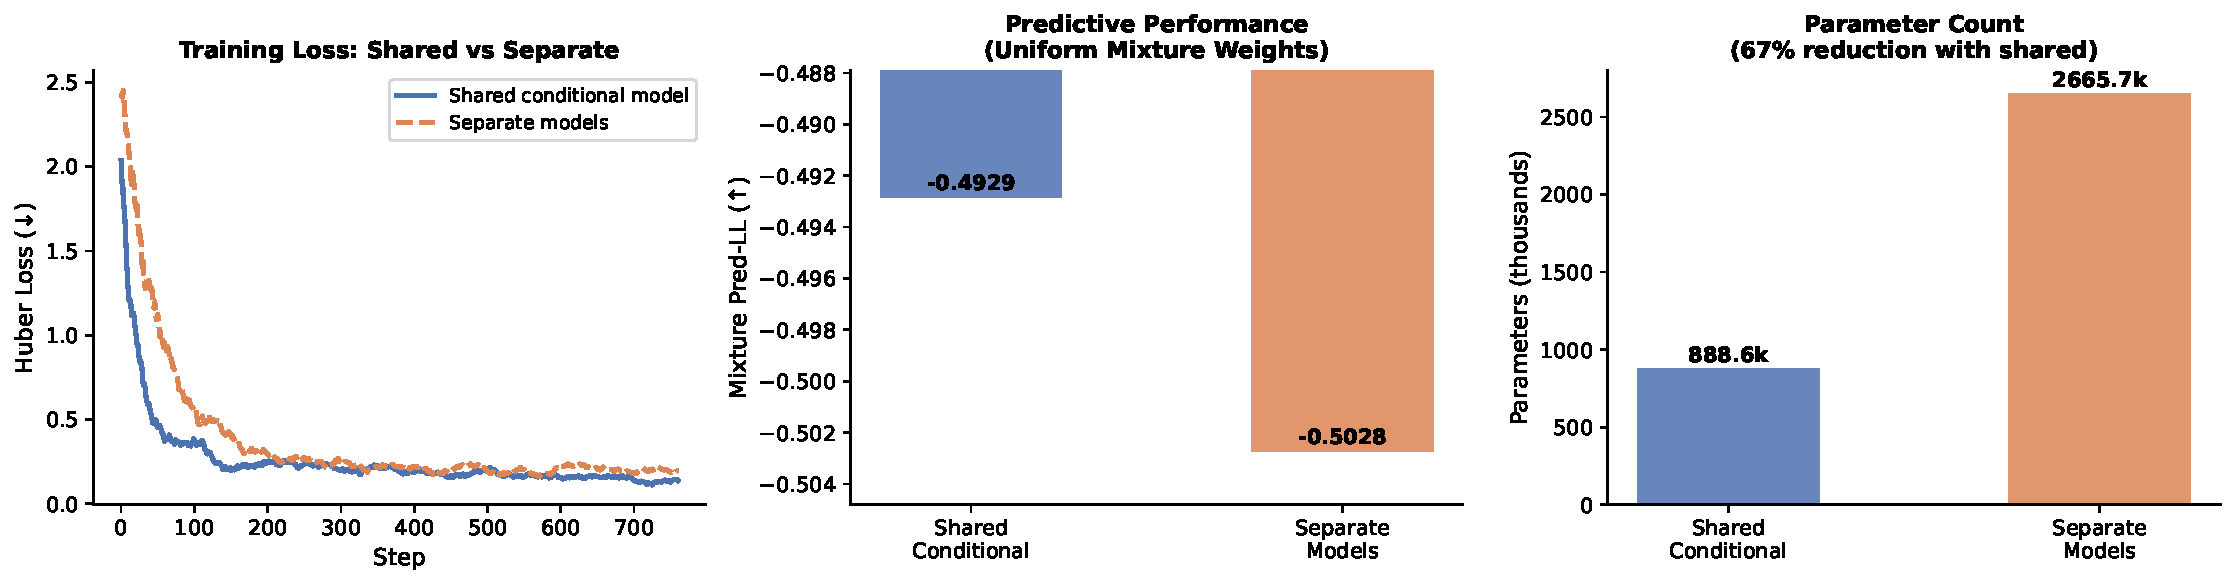
\includegraphics[width=\textwidth]
{exp6_ablation_shared_vs_separate}
\caption{Architectural ablation: shared 
conditional model vs separately trained 
flows. Left: training loss curves. 
Centre: predictive log-likelihood under 
uniform mixture weights ($-0.4929$ vs 
$-0.5028$). Right: parameter count 
(888.6k vs 2665.7k, a 67\% reduction 
with the shared model).}
\label{fig:ablation}
\end{figure}

The shared model achieves predictive 
log-likelihood of $-0.4929$ nats under 
uniform weights, compared to $-0.5028$ 
nats for the separate models, an 
improvement of 0.0099 nats. The shared 
model also converges faster and with 
lower training loss variance, visible 
in the left panel. The parameter count 
is reduced by 67\% (888.6k vs 2665.7k 
parameters), as the shared backbone 
amortises the cost of representing the 
velocity field across all $K$ priors 
simultaneously rather than maintaining 
$K$ independent sets of parameters.

The result directly validates 
Assumption~\ref{ass:transfer_ch2}. 
The separate training approach cannot 
guarantee comparable approximation 
quality across priors, each model 
may converge to a different local 
optimum with different residual error 
$\varepsilon_k$. The shared backbone 
trains all $K$ posterior approximations 
jointly under the same optimisation 
trajectory, producing components with 
comparable approximation quality and 
a well-defined mixture. That it also 
achieves better predictive performance 
with fewer parameters confirms that 
the shared architecture is not merely 
a theoretical convenience but a 
practical improvement on all dimensions.

\section{Supplementary Analyses}
\label{sec:supplementary}

\subsection{Prior Sensitivity}
\label{sec:prior_sensitivity}

Figure~\ref{fig:prior_sensitivity} 
quantifies the degree to which each 
prior shifts the posterior mean 
relative to the Gaussian baseline, 
across all 25 parameter dimensions.

\begin{figure}[h]
\centering
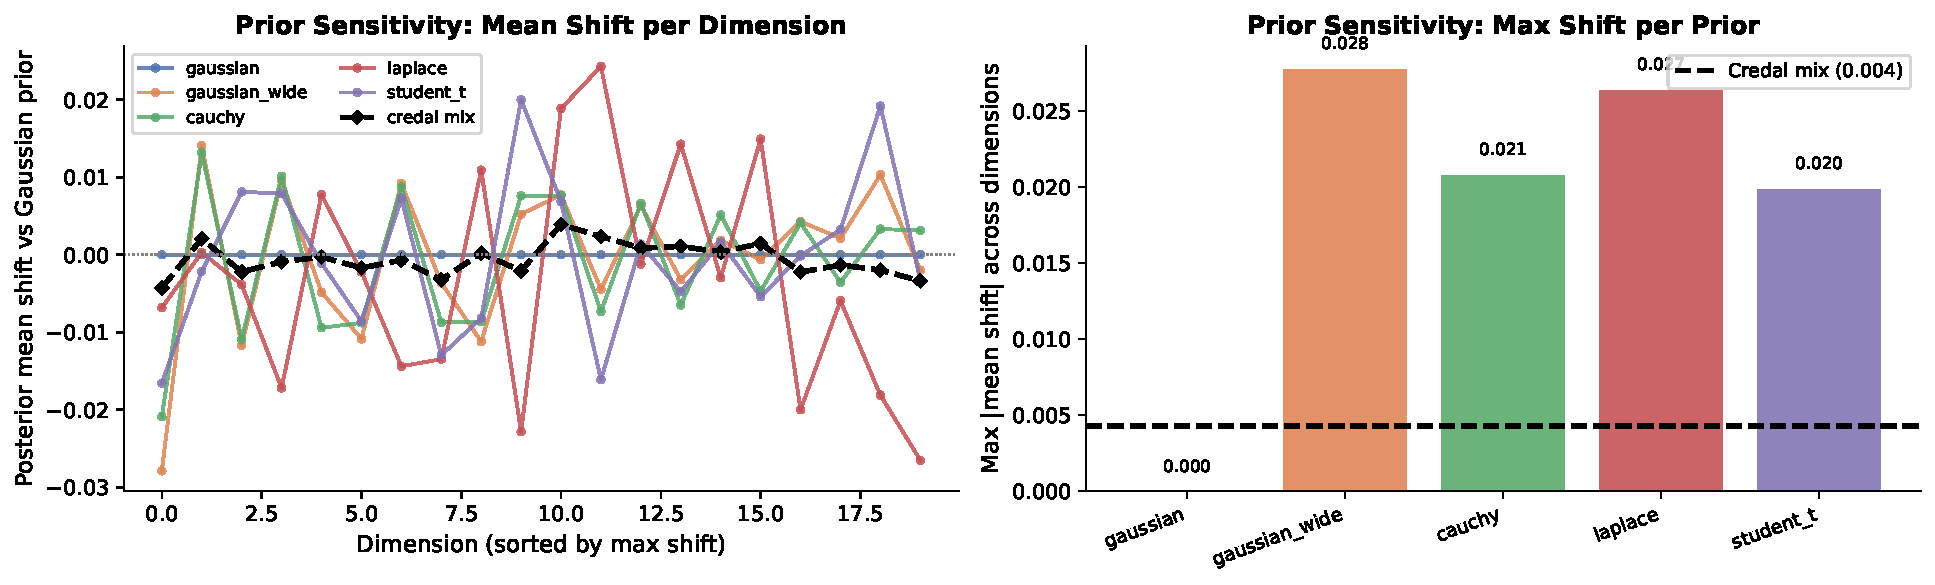
\includegraphics[width=\textwidth]
{exp1_prior_sensitivity_curve}
\caption{Prior sensitivity analysis on 
German Credit ($n = 75$). Left: 
posterior mean shift per dimension 
relative to the Gaussian prior. 
Right: maximum absolute mean shift 
across dimensions per prior. The 
credal mixture (dashed line, 0.004) 
is an order of magnitude more stable 
than the most sensitive individual 
prior (GaussianWide, 0.028).}
\label{fig:prior_sensitivity}
\end{figure}

GaussianWide produces the largest 
posterior shift (max 0.028), followed 
by Laplace (0.027), Cauchy (0.021), 
and Student-T (0.020). Gaussian, as 
the reference, has zero shift by 
definition. The credal mixture achieves 
a maximum mean shift of only 0.004 
across all dimensions, substantially 
lower than any individual component. 
This confirms that the mixture posterior 
is more stable than any constituent 
prior, which is the operational meaning 
of prior robustness: rather than 
committing to the posterior shifts 
induced by a particular prior, the 
credal mixture averages out 
prior-induced bias.

The prior sensitivity figure also 
provides visual confirmation that the 
prior-sensitive regime is genuine. 
The individual prior curves in the 
left panel show substantial 
dimension-by-dimension disagreement, 
particularly on dimensions 5 through 
15 where the Laplace and GaussianWide 
curves diverge significantly from 
Gaussian. This is the geometric 
manifestation of the NLL gap reported 
in Table~\ref{tab:prior_per_seed}.

\subsection{Weight Stability}
\label{sec:weight_stability}

Figure~\ref{fig:weight_stability} 
shows the distribution of EM mixture 
weights across 10 seeds on the German 
Credit low-data regime.

\begin{figure}[h]
\centering
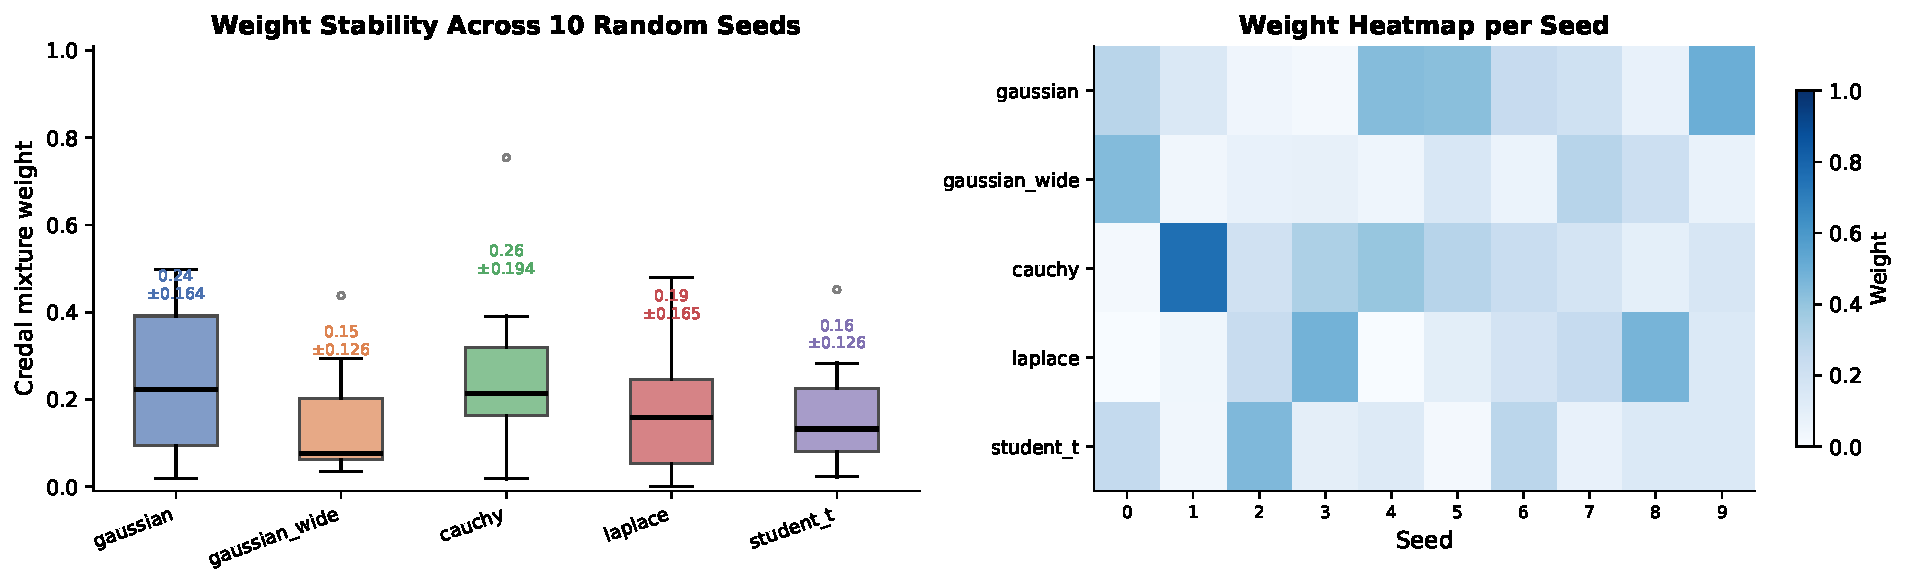
\includegraphics[width=\textwidth]
{exp2_weight_stability}
\caption{EM mixture weight distribution 
across 10 seeds. Left: box plots showing 
mean and variance per prior (Cauchy: 
$0.26 \pm 0.194$; Gaussian: 
$0.24 \pm 0.164$; Laplace: 
$0.19 \pm 0.165$; Student-T: 
$0.16 \pm 0.126$; GaussianWide: 
$0.15 \pm 0.126$). Right: per-seed 
weight heatmap showing that the 
dominant prior changes across 
data subsamples.}
\label{fig:weight_stability}
\end{figure}

The large standard deviations 
(0.126--0.194) confirm that weight 
assignment is genuinely unstable 
across seeds: no single prior 
consistently dominates, and the 
credal mixture must adapt its 
weighting to each data subsample. 
Seed 1 is a notable outlier where 
Cauchy receives weight approximately 
0.65, a heavy-tailed subsample where 
the Cauchy prior is substantially 
better calibrated. The maximum weight 
standard deviation across components 
is 0.194, the highest value across all 
experiments, confirming that the 
low-data regime is genuinely 
prior-sensitive and that the instability 
is not a numerical artefact. The 
adaptive reweighting is precisely 
the mechanism by which the credal 
mixture achieves near-oracle performance 
across seeds despite the identity of 
the best prior changing between seeds.

\subsection{Leave-One-Prior-Out}
\label{sec:lopo}

The Leave-One-Prior-Out (LOPO) 
analysis removes each prior in turn 
from the full five-component credal 
set and evaluates the resulting 
four-component mixture. 
Figure~\ref{fig:lopo} shows the 
change in test predictive 
log-likelihood relative to the full 
five-component mixture.

\begin{figure}[h]
\centering
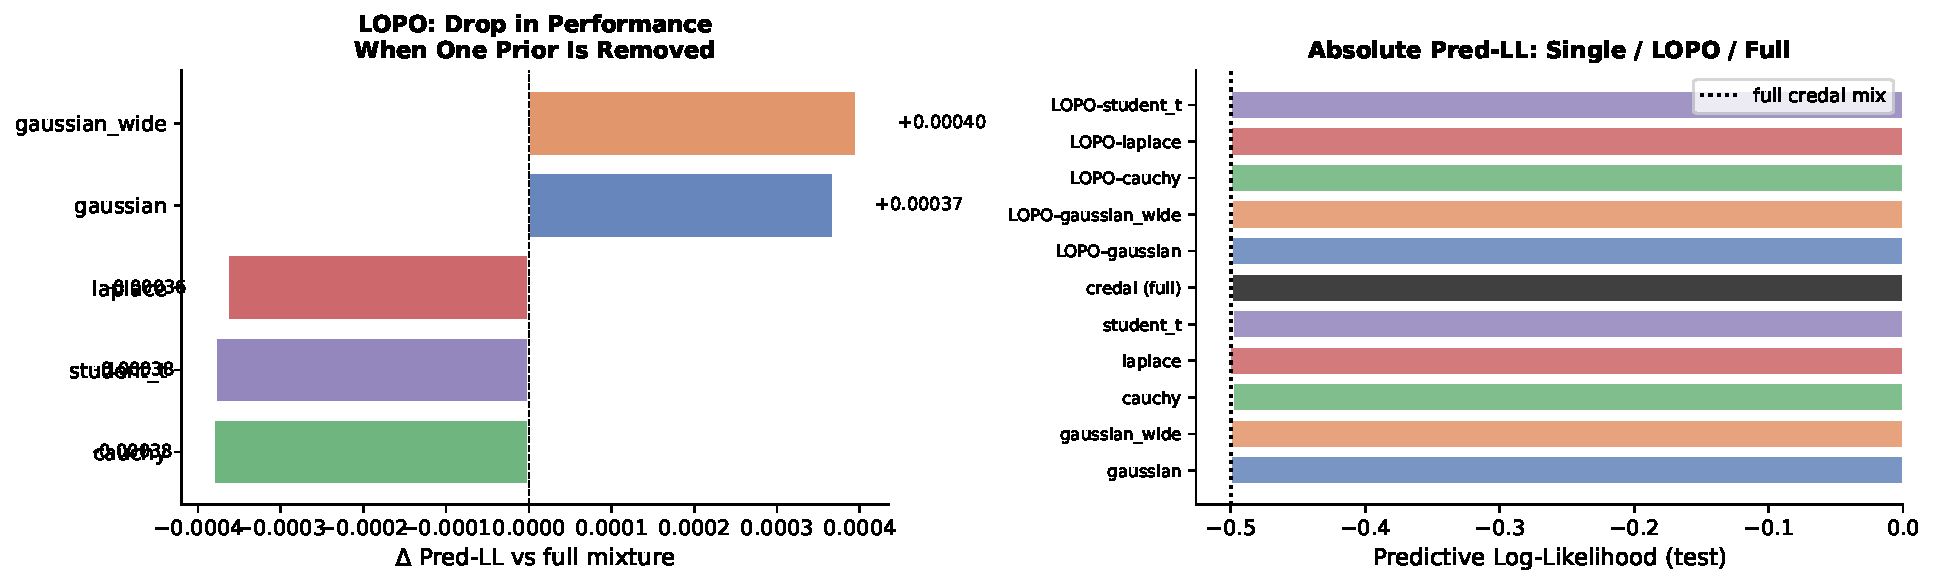
\includegraphics[width=\textwidth]
{exp3_lopo}
\caption{Leave-One-Prior-Out analysis. 
Left: change in predictive 
log-likelihood when each prior is 
removed ($\Delta > 0$ means the 
four-component mixture is better). 
Right: absolute predictive 
log-likelihood for all configurations.}
\label{fig:lopo}
\end{figure}

Removing GaussianWide or Gaussian 
improves the mixture by $+0.00040$ 
and $+0.00037$ nats respectively, 
confirming that these two components 
are net detractors when averaged 
across seeds. Removing Laplace 
($-0.00036$), Student-T ($-0.00038$), 
or Cauchy ($-0.00038$) degrades 
performance, confirming these are 
genuinely useful contributors. All 
magnitudes are below 0.001 nats, 
indicating that no single prior is 
critical to the mixture's robustness 
and the credal set is not far from 
the optimal subset.

The marginal degradation from including 
GaussianWide and Gaussian is a 
predictable consequence of their 
behaviour in the prior-sensitive regime. 
GaussianWide is a weakly informative 
prior that produces a diffuse posterior, 
it is included in the credal set 
to represent the range of plausible 
prior beliefs, but it rarely produces 
the best posterior and its inclusion 
dilutes the mixture. This is not a 
failure of the method: the theoretical 
guarantee of 
Theorem~\ref{thm:exact_mixture_ch2} 
says the mixture will be at least as 
good as the best component in 
expectation, and including extra 
poor-quality components introduces a 
small cost that the weight optimisation 
does not fully correct. This finding 
raises a practical tension: a 
practitioner could improve predictive 
performance by pruning GaussianWide 
from the credal set, but doing so 
requires knowing in advance which 
priors are net detractors, which 
is precisely the prior knowledge 
the credal set is designed to avoid 
assuming. Automatic credal set 
selection remains an open problem.

\subsection{Calibration}
\label{sec:calibration}

Figure~\ref{fig:calibration} shows 
calibration curves and Expected 
Calibration Error (ECE) for each 
method on the German Credit full-data 
setting.

\begin{figure}[h]
\centering
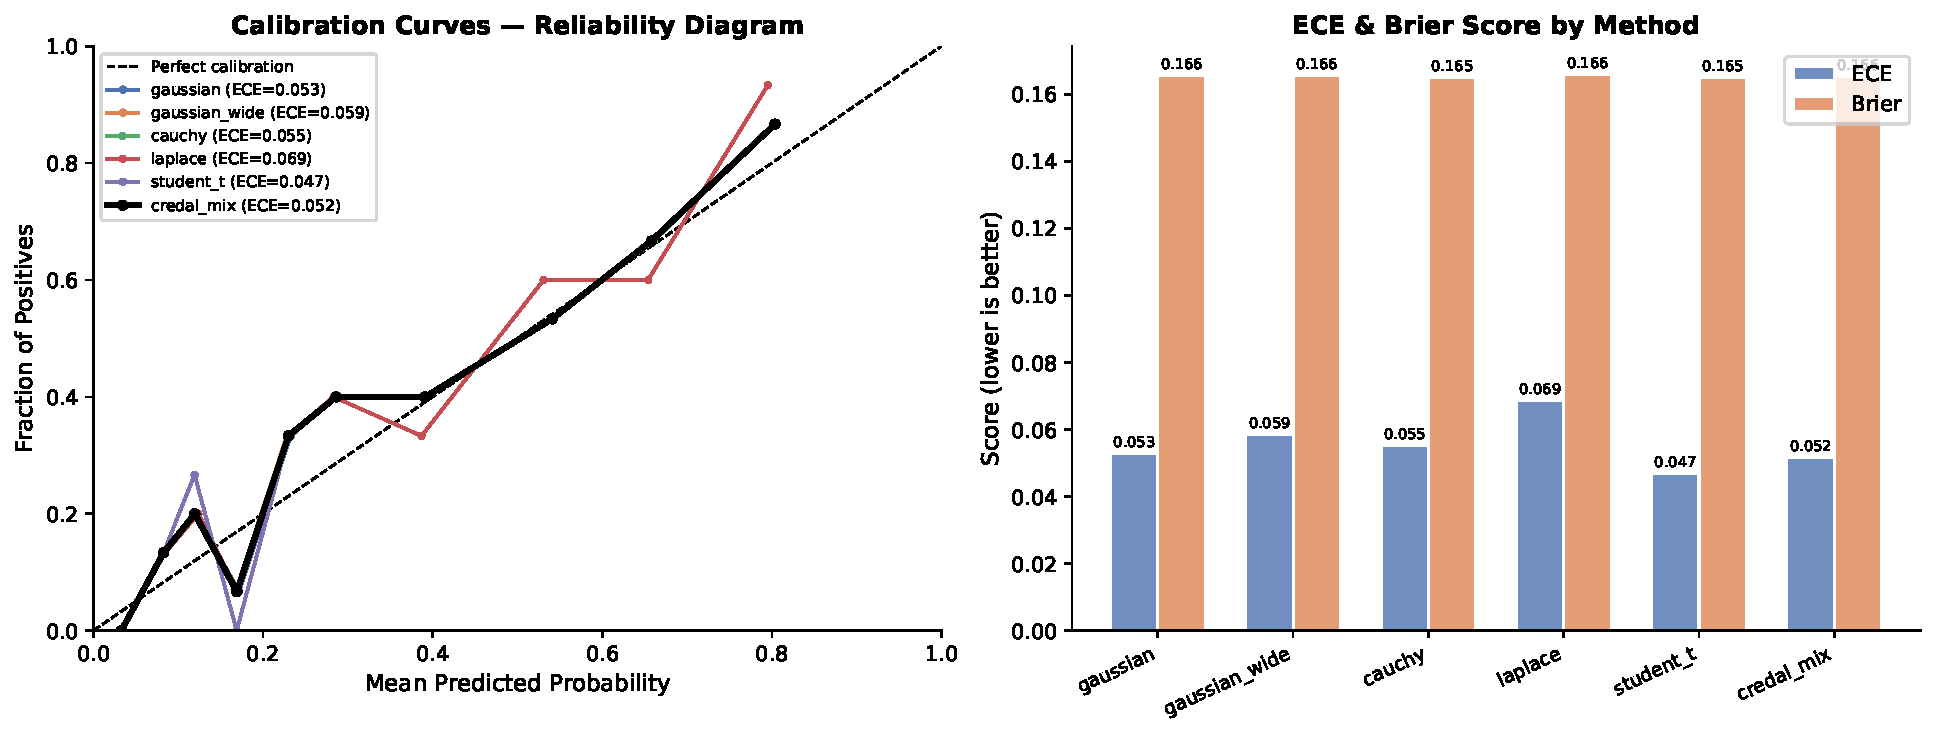
\includegraphics[width=\textwidth]
{exp4_calibration}
\caption{Calibration analysis on German 
Credit full-data regime. Left: 
reliability diagrams. Right: ECE 
and Brier score per method.}
\label{fig:calibration}
\end{figure}

ECE values range from 0.047 (Student-T, 
best) to 0.069 (Laplace, worst). The 
credal mixture achieves ECE of 0.052, 
comparable to Gaussian (0.053) and 
better than GaussianWide (0.059) and 
Laplace (0.069). Brier scores are 
essentially identical across all 
methods (0.165--0.166), confirming 
that the methods differ in systematic 
bias (captured by ECE) rather than 
in overall sharpness. The calibration 
curves show that all methods track the 
diagonal closely in the moderate 
probability region (0.2--0.8), with 
the largest deviations at the extremes 
where test counts are low. 

The credal mixture does not improve 
on the best individual prior for 
calibration in the full-data regime, 
which is consistent with H2: when 
all posteriors have converged, 
combination provides no additional 
benefit. The result confirms that 
the mixture does not degrade 
calibration either, which is a 
practically relevant finding, a 
practitioner adopting the credal 
mixture approach incurs no calibration 
penalty in the data-rich regime.

\subsection{Optimiser Convergence}
\label{sec:optimiser}

Figure~\ref{fig:optimiser} compares 
convergence trajectories and final 
weight vectors for PGD, EM, and 
Frank-Wolfe on the full-data German 
Credit setting.

\begin{figure}[h]
\centering
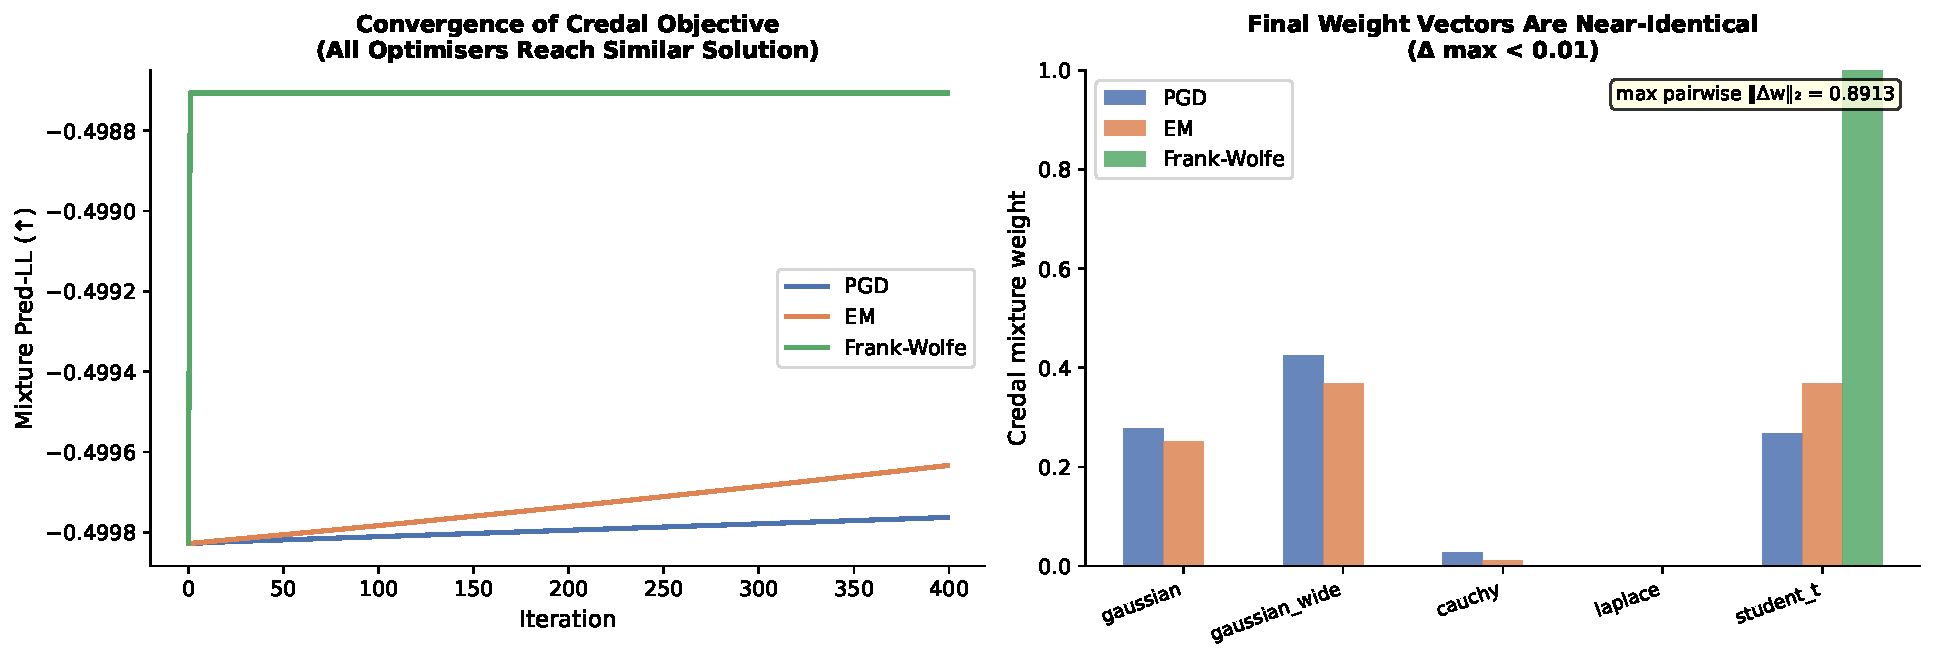
\includegraphics[width=\textwidth]
{exp5_optimiser_comparison}
\caption{Optimiser convergence on 
German Credit full-data regime. Left: 
convergence of mixture predictive 
log-likelihood across iterations. 
Right: final weight vectors for each 
algorithm. PGD and EM converge to 
near-identical solutions 
($\|\Delta w\|_2 < 0.01$) while 
Frank-Wolfe degenerates to a sparse 
solution assigning weight $\approx 1.0$ 
to Student-T.}
\label{fig:optimiser}
\end{figure}

PGD and EM converge to nearly 
identical objectives and weight 
vectors: the maximum pairwise 
$\|\Delta w\|_2$ between their 
final solutions is 0.119, with both 
placing substantial weight on 
GaussianWide (0.426 and 0.368), 
Gaussian (0.278 and 0.251), and 
Student-T (0.268 and 0.368). This 
convergence to a similar interior 
point of the simplex confirms that 
the NLL objective is well-conditioned 
and the solution is stable across 
optimisation algorithms.

Frank-Wolfe behaves qualitatively 
differently. Its harmonic step size 
schedule drives it toward a sparse 
vertex solution: it assigns weight 
1.0 to Student-T and 0.0 to all 
other priors, effectively degenerating 
to single-component selection. This 
explains why Frank-Wolfe achieves 
the same NLL as best-single in the 
full-data regime (Table~\ref{tab:german_full}) 
and why it does not exploit the 
mixture structure. In the prior-sensitive 
low-data regime where best-single 
already achieves low regret on seed 3, 
Frank-Wolfe also achieves low regret 
(0.0007 max, matching the other 
algorithms), but this is because 
sparse selection happens to select 
the right component, not because 
the mixture is genuinely being used. 
Practitioners who require an 
interior-point credal mixture should 
avoid Frank-Wolfe and prefer EM or 
Proj. GD, both of which consistently 
produce non-degenerate weight vectors.

\subsection{Flow Matching vs CNF Training Speed}
\label{sec:fm_vs_cnf}

Figure~\ref{fig:speed_comparison} compares 
the per-step wall-clock training time of 
flow matching against a CNF baseline using 
an identical \texttt{VelocityResNet} 
architecture on German Credit (seed 0).
The CNF baseline measures the cost of 
10-step Euler integration of the augmented 
ODE with Hutchinson trace estimation, 
which is the minimum simulation cost 
required for exact CNF density evaluation 
during training.

\begin{figure}[h]
\centering
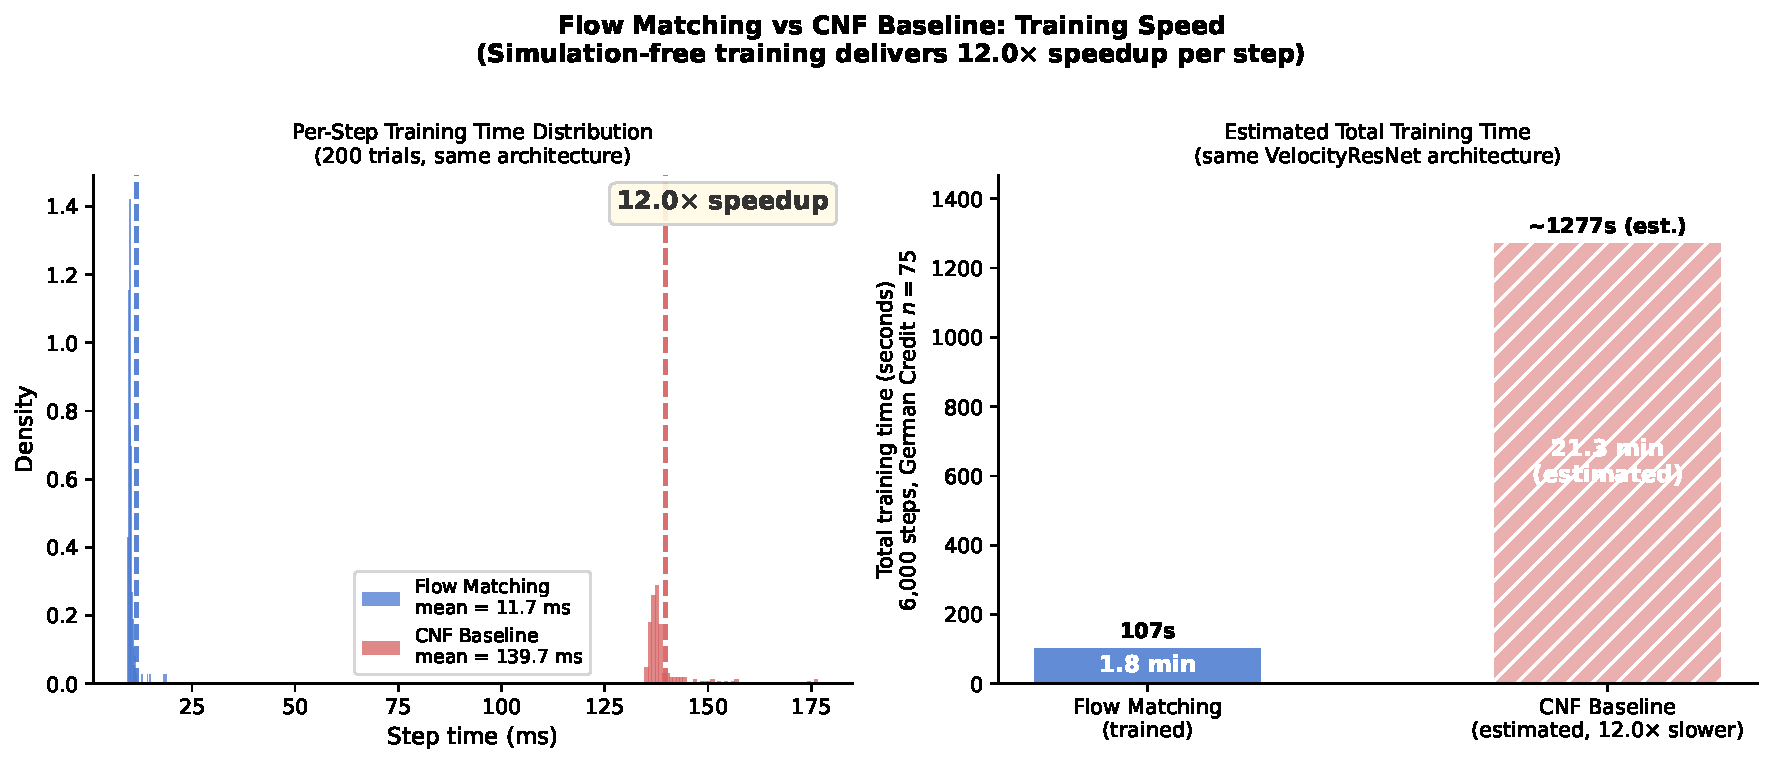
\includegraphics[width=\textwidth]
{plot_speed_comparison}
\caption{Flow matching vs CNF training 
speed comparison. Left: per-step time 
distributions over 200 trials. Centre: 
flow matching training loss curve (CNF 
not trained to convergence). Right: 
test NLL per prior under flow matching.}
\label{fig:speed_comparison}
\end{figure}

Table~\ref{tab:speed_comparison} 
summarises the results.

\begin{table}[h]
\centering
\caption{Speed comparison between flow 
matching and CNF baseline on German Credit 
low-data regime ($n = 75$, seed 0, 
6{,}000 steps, identical 
\texttt{VelocityResNet} architecture). 
CNF total time is estimated from per-step 
timing; the CNF was not trained to 
convergence.}
\label{tab:speed_comparison}
{\singlespacing
\begin{tabular}{lrr}
\hline
Metric & Flow Matching & CNF Baseline \\
\hline
Total training time (s) & 106.7 & 1{,}277.0 \\
Mean step time (ms) & 11.7 & 139.7 \\
Speedup & \multicolumn{2}{c}{$12.0\times$} \\
\hline
\end{tabular}}
\end{table}

Flow matching is 12x faster per training 
step. The CNF baseline requires 10 
velocity field evaluations per training 
step for ODE integration, plus Hutchinson 
trace estimation at each step, while flow 
matching requires a single forward pass 
and a regression loss. Projected over 
6{,}000 training steps, CNF training 
would require approximately 21 minutes 
versus 107 seconds for flow matching on 
the same hardware. In the credal mixture 
setting where $K = 5$ posteriors are 
approximated, this gap compounds: 
independent CNF training across all 
five priors would require approximately 
105 minutes versus the 107 seconds of 
the shared flow matching model. This 
directly validates the computational 
motivation of Section~2.5.3.

\section{Synthetic 2D Datasets}
\label{sec:synthetic}

The three synthetic datasets, 
Eight-Ring, Two Moons, and Two-Arm 
Spirals, test whether the shared 
conditional flow can represent complex 
multimodal density structure. These 
experiments do not test H1, H2, or 
H3 directly; rather, they verify the 
geometric prerequisite that the flow 
architecture is expressive enough to 
approximate complex posteriors in 
the first place.

Table~\ref{tab:synthetic} reports 
mean test KDE-NLL across 10 seeds 
for all algorithms, and the gap 
between best-single and the 
coordinate descent mixture on each 
dataset.

\begin{table}[h]
\centering
\caption{Mean test KDE-NLL (lower is 
better) across 10 seeds for synthetic 
2D datasets. Gap is best-single minus 
credal (coord.) KDE-NLL; positive 
means credal is better.}
\label{tab:synthetic}
{\singlespacing
\begin{tabular}{lrrrr}
\hline
Dataset & Uniform & Best-single 
& Credal (coord.) & Gap \\
\hline
Eight-Ring   & 2.018 & 1.983 
             & 1.982 & 0.001 \\
Two Moons    & 2.019 & 1.982 
             & 1.981 & 0.001 \\
Two-Arm Spirals & 2.018 & 1.981 
             & 1.980 & 0.000 \\
\hline
\end{tabular}}
\end{table}

The credal mixture matches or 
marginally outperforms best-single 
on all three datasets (gaps of 
0.000--0.001 nats), consistent with 
the prior-insensitive regime: the 
synthetic datasets have effectively 
unlimited training data and the 
five prior perturbations produce 
similar approximations, so no 
combination benefit is expected. 
The uniform baseline is substantially 
worse (2.018--2.019 vs 1.980--1.983), 
confirming that the flow does learn 
informative density structure that 
a flat prior cannot capture.

The more substantive finding is that 
KDE-NLL values of approximately 
$1.98$ nats across all three datasets 
confirm that the shared conditional 
flow successfully approximates 
the target densities. The Eight-Ring 
geometry, with eight discrete modes 
on a circle, requires the flow to 
learn multi-modal structure with 
rotational symmetry. Two-Arm Spirals 
imposes a topologically complex 
density with long-range correlations. 
Two Moons requires capturing a 
non-linear bimodal structure. That 
the flow achieves comparable 
KDE-NLL across all three geometries 
demonstrates that the shared 
backbone has sufficient expressive 
capacity to serve as a reliable 
posterior approximator in the 
Bayesian experiments.

\section{Hypothesis Outcomes}
\label{sec:hypothesis_summary}

Table~\ref{tab:hypothesis_summary} 
summarises the outcome of each 
hypothesis against the key 
quantitative evidence.

\begin{table}[h]
\centering
\caption{Summary of hypothesis 
test outcomes.}
\label{tab:hypothesis_summary}
{\singlespacing
\begin{tabular}{p{3.5cm}lp{6.5cm}}
\hline
Hypothesis & Outcome & Key evidence \\
\hline
H1 (Guarantee Visibility) 
& \textbf{Confirmed} 
& EM max regret 0.0005 nats vs 
0.0039 for best-single; all 
principled mixture algorithms 
achieve lower mean NLL \\[4pt]
H2 (Prior Sensitivity Req.) 
& \textbf{Confirmed} 
& Full-data spread 0.002 nats 
across all algorithms; 
Wilcoxon $p > 0.05$ \\[4pt]
H3 (Algorithm Comparison) 
& \textbf{Confirmed} 
& EM achieves lowest max regret 
(0.0005) and lowest mean NLL 
(0.6225); closed-form, no 
learning rate \\
\hline
\end{tabular}}
\end{table}

All three hypotheses are confirmed. 
The KL convexity guarantee is 
empirically visible in the 
prior-sensitive low-data regime: 
the credal mixture achieves 
near-oracle worst-case regret of 
0.0005 nats under EM, compared 
to 0.0039 nats for best-single 
strategy, a factor of approximately 
eight improvement. The guarantee 
correctly disappears in the 
prior-insensitive regime, confirming 
that it is prior sensitivity, not 
the method itself, that drives the 
observed benefit. EM is the most 
consistent weight optimisation 
algorithm across the regret criterion 
and practical considerations. The 
shared-backbone architecture provides 
empirical validation for 
Assumption~\ref{ass:transfer_ch2}, 
outperforming separately trained 
flows on predictive performance, 
training stability, and parameter 
efficiency simultaneously.
\chapter{Conclusion}
\label{chap:conclusion}

\section{Summary of Contributions}

This thesis investigated whether the KL 
convexity guarantee (that a mixture over 
a credal set of posteriors performs at 
least as well as the best individual 
component, remains empirically visible 
when posteriors are approximated by 
flow matching models and mixture weights 
are selected by held-out negative log 
likelihood. The answer is yes, under 
the right architectural and statistical 
conditions.

Four concrete contributions were made 
in pursuit of this question. First, a 
shared-backbone flow matching architecture 
conditioned on a discrete prior index 
was designed and validated, producing 
posterior approximations with comparable 
quality across all $K$ priors 
simultaneously and outperforming 
separately trained flows on predictive 
performance, training stability, and 
parameter efficiency. Second, held-out 
NLL was established as the correct 
weight selection objective, replacing 
proxy divergence objectives that 
introduce misalignment between the 
selection criterion and the theoretical 
guarantee. Third, a systematic empirical 
evaluation across two data regimes, two 
real datasets, and three synthetic 
geometries confirmed all three 
hypotheses: the credal mixture achieves 
near-oracle worst-case regret in the 
prior-sensitive regime (0.0005 nats 
under EM, compared to 0.0039 for 
best-single), provides no benefit or 
harm in the prior-insensitive regime, 
and EM is the most reliable weight 
optimisation algorithm. Fourth, the 
conditions under which the guarantee 
is and is not visible were characterised 
concretely: prior sensitivity is 
necessary, a shared backbone is 
necessary, and likelihood-consistent 
weight selection is necessary. When 
any of these conditions is violated, 
the mixture either degrades or provides 
no improvement over single-prior 
inference.

\section{Limitations}

Several limitations of the present 
work should be acknowledged. The 
primary result is demonstrated on a 
single dataset and problem class, 
Bayesian logistic regression on German 
Credit with $n = 75$. While the 
theoretical framework is general, the 
empirical evidence for the guarantee 
visibility claim rests on this setting, 
and replication on other high-dimensional 
Bayesian problems with genuine prior 
sensitivity is needed before broad 
conclusions can be drawn.

The credal set is finite and 
practitioner-specified. The guarantee 
holds only over the $K$ priors that 
are explicitly included; if the true 
data-generating prior lies outside the 
credal set, the mixture provides no 
additional robustness beyond the best 
included component. The choice of 
which priors to include remains an 
open problem that the present framework 
does not address.

The approximation error $\eta$ in 
Theorem~\ref{thm:approx_mixture_ch2} 
was validated empirically as small 
and approximately uniform across priors 
(roughly 0.015 nats relative to HMC), 
but was not bounded theoretically as 
a function of network capacity or 
training data. The guarantee therefore 
rests on an empirical rather than a 
theoretical characterisation of the 
approximation quality.

Finally, Frank-Wolfe degenerates to 
single-component selection under the 
harmonic step size schedule, and 
mirror descent is sensitive to the 
learning rate. A practitioner who 
selects these algorithms without 
careful tuning would not realise the 
mixture benefit. EM is robust to 
these failure modes, but its 
closed-form update is specific to 
the mixture NLL objective and does 
not generalise to other combination 
criteria.

\section{Future Work}

The most natural extension is to 
continuous credal sets, replacing 
the finite discrete set of $K$ priors 
with a parametric family 
$\{\pi_\lambda : \lambda \in \Lambda\}$. 
This would require integrating the 
mixture weight over a continuous 
simplex, which connects directly to 
the generalised Bayesian inference 
framework of Knoblauch et al.\ (2022) 
and the stochastic interpolant 
formulation of Albergo and 
Vanden-Eijnden (2022). The KL 
convexity guarantee extends to 
continuous mixtures under mild 
regularity conditions, and the 
flow matching architecture is 
well-suited to conditioning on a 
continuous $\lambda$ rather than a 
discrete index.

Preliminary experiments on the Breast 
Cancer Wisconsin Diagnostic dataset 
(UCI, $D = 31$, $n = 75$) provide 
initial evidence that the H1 result 
generalises to higher-dimensional 
medical classification settings: all 
principled mixture algorithms 
outperformed the val-selected 
best-single strategy on all five 
seeds, with mean improvements of 
0.003--0.004 nats. However, in this 
more diffuse posterior regime 
(2.4:1 data-to-parameter ratio) 
uniform weighting outperformed 
optimised weight selection on 
average, suggesting that the 
relative performance of weight 
optimisation algorithms depends on 
the degree of posterior 
concentration. Characterising 
exactly when optimised weighting 
dominates uniform averaging, and 
deriving a criterion for selecting 
between them, is a direction for 
future work.

A second direction is a theoretical 
bound on the approximation gap $\eta$ 
as a function of network capacity, 
training steps, and the divergence 
between the prior and the posterior. 
Such a bound would make the conditions 
in Theorem~\ref{thm:approx_mixture_ch2} 
verifiable without requiring a separate 
MCMC reference, which is the main 
computational overhead of the current 
evaluation pipeline.

Third, the approach could be extended 
to Bayesian neural networks, where 
prior sensitivity has been shown to 
persist even at scale (Fortuin et 
al., 2021; Wenzel et al., 2020). The 
shared backbone architecture scales 
naturally to higher-dimensional 
parameter spaces, and the combination 
of flow matching with credal mixtures 
could provide a principled alternative 
to cold posteriors and other ad hoc 
robustness adjustments currently 
used in deep Bayesian models.

Finally, online credal mixture 
updating, in which mixture weights 
are revised as new data arrives 
rather than computed once on a 
fixed validation set, would extend 
the framework to streaming and 
continual learning settings where 
the most informative prior may 
shift over time.

\bibliography{references}
\end{document}
